% Options for packages loaded elsewhere
\PassOptionsToPackage{unicode}{hyperref}
\PassOptionsToPackage{hyphens}{url}
\PassOptionsToPackage{dvipsnames,svgnames,x11names}{xcolor}
%
\documentclass[
]{aft}

\usepackage{amsmath,amssymb}
\usepackage{iftex}
\ifPDFTeX
  \usepackage[T1]{fontenc}
  \usepackage[utf8]{inputenc}
  \usepackage{textcomp} % provide euro and other symbols
\else % if luatex or xetex
  \usepackage{unicode-math}
  \defaultfontfeatures{Scale=MatchLowercase}
  \defaultfontfeatures[\rmfamily]{Ligatures=TeX,Scale=1}
\fi
\usepackage{lmodern}
\ifPDFTeX\else  
    % xetex/luatex font selection
\fi
% Use upquote if available, for straight quotes in verbatim environments
\IfFileExists{upquote.sty}{\usepackage{upquote}}{}
\IfFileExists{microtype.sty}{% use microtype if available
  \usepackage[]{microtype}
  \UseMicrotypeSet[protrusion]{basicmath} % disable protrusion for tt fonts
}{}
\makeatletter
\@ifundefined{KOMAClassName}{% if non-KOMA class
  \IfFileExists{parskip.sty}{%
    \usepackage{parskip}
  }{% else
    \setlength{\parindent}{0pt}
    \setlength{\parskip}{6pt plus 2pt minus 1pt}}
}{% if KOMA class
  \KOMAoptions{parskip=half}}
\makeatother
\usepackage{xcolor}
\setlength{\emergencystretch}{3em} % prevent overfull lines
\setcounter{secnumdepth}{5}
% Make \paragraph and \subparagraph free-standing
\makeatletter
\ifx\paragraph\undefined\else
  \let\oldparagraph\paragraph
  \renewcommand{\paragraph}{
    \@ifstar
      \xxxParagraphStar
      \xxxParagraphNoStar
  }
  \newcommand{\xxxParagraphStar}[1]{\oldparagraph*{#1}\mbox{}}
  \newcommand{\xxxParagraphNoStar}[1]{\oldparagraph{#1}\mbox{}}
\fi
\ifx\subparagraph\undefined\else
  \let\oldsubparagraph\subparagraph
  \renewcommand{\subparagraph}{
    \@ifstar
      \xxxSubParagraphStar
      \xxxSubParagraphNoStar
  }
  \newcommand{\xxxSubParagraphStar}[1]{\oldsubparagraph*{#1}\mbox{}}
  \newcommand{\xxxSubParagraphNoStar}[1]{\oldsubparagraph{#1}\mbox{}}
\fi
\makeatother


\providecommand{\tightlist}{%
  \setlength{\itemsep}{0pt}\setlength{\parskip}{0pt}}\usepackage{longtable,booktabs,array}
\usepackage{calc} % for calculating minipage widths
% Correct order of tables after \paragraph or \subparagraph
\usepackage{etoolbox}
\makeatletter
\patchcmd\longtable{\par}{\if@noskipsec\mbox{}\fi\par}{}{}
\makeatother
% Allow footnotes in longtable head/foot
\IfFileExists{footnotehyper.sty}{\usepackage{footnotehyper}}{\usepackage{footnote}}
\makesavenoteenv{longtable}
\usepackage{graphicx}
\makeatletter
\def\maxwidth{\ifdim\Gin@nat@width>\linewidth\linewidth\else\Gin@nat@width\fi}
\def\maxheight{\ifdim\Gin@nat@height>\textheight\textheight\else\Gin@nat@height\fi}
\makeatother
% Scale images if necessary, so that they will not overflow the page
% margins by default, and it is still possible to overwrite the defaults
% using explicit options in \includegraphics[width, height, ...]{}
\setkeys{Gin}{width=\maxwidth,height=\maxheight,keepaspectratio}
% Set default figure placement to htbp
\makeatletter
\def\fps@figure{htbp}
\makeatother

\usepackage{booktabs}
\usepackage{longtable}
\usepackage{array}
\usepackage{multirow}
\usepackage{wrapfig}
\usepackage{float}
\usepackage{colortbl}
\usepackage{pdflscape}
\usepackage{tabu}
\usepackage{threeparttable}
\usepackage{threeparttablex}
\usepackage[normalem]{ulem}
\usepackage{makecell}
\usepackage{xcolor}
\usepackage{orcidlink}
\definecolor{mypink}{RGB}{219, 48, 122}
\makeatletter
\@ifpackageloaded{caption}{}{\usepackage{caption}}
\AtBeginDocument{%
\ifdefined\contentsname
  \renewcommand*\contentsname{Table of contents}
\else
  \newcommand\contentsname{Table of contents}
\fi
\ifdefined\listfigurename
  \renewcommand*\listfigurename{List of Figures}
\else
  \newcommand\listfigurename{List of Figures}
\fi
\ifdefined\listtablename
  \renewcommand*\listtablename{List of Tables}
\else
  \newcommand\listtablename{List of Tables}
\fi
\ifdefined\figurename
  \renewcommand*\figurename{Figure}
\else
  \newcommand\figurename{Figure}
\fi
\ifdefined\tablename
  \renewcommand*\tablename{Table}
\else
  \newcommand\tablename{Table}
\fi
}
\@ifpackageloaded{float}{}{\usepackage{float}}
\floatstyle{ruled}
\@ifundefined{c@chapter}{\newfloat{codelisting}{h}{lop}}{\newfloat{codelisting}{h}{lop}[chapter]}
\floatname{codelisting}{Listing}
\newcommand*\listoflistings{\listof{codelisting}{List of Listings}}
\makeatother
\makeatletter
\makeatother
\makeatletter
\@ifpackageloaded{caption}{}{\usepackage{caption}}
\@ifpackageloaded{subcaption}{}{\usepackage{subcaption}}
\makeatother

\ifLuaTeX
  \usepackage{selnolig}  % disable illegal ligatures
\fi
\usepackage[]{natbib}
\bibliographystyle{te}
\usepackage{bookmark}

\IfFileExists{xurl.sty}{\usepackage{xurl}}{} % add URL line breaks if available
\urlstyle{same} % disable monospaced font for URLs
\hypersetup{
  pdftitle={Modeling Longitudinal Binary Outcomes in a Small Matched-Pair Sample with Application to Cardiovascular Data: A Simulation Study},
  pdfauthor={Jinyu Luo; Chun-Po Steve Fan; Sudipta Saha; Aya Mitani},
  pdfkeywords={GEE, QLS, Longitudinal},
  colorlinks=true,
  linkcolor={blue},
  filecolor={Maroon},
  citecolor={Blue},
  urlcolor={red},
  pdfcreator={LaTeX via pandoc}}



\title{Modeling Longitudinal Binary Outcomes in a Small Matched-Pair
Sample with Application to Cardiovascular Data: A Simulation Study}
\author{
Jinyu Luo~\orcidlink{0009-0004-1101-7040}\\University of
Toronto\\\href{mailto:jinyu.luo@mail.utoronto.ca}{jinyu.luo@mail.utoronto.ca}\and 
Chun-Po Steve Fan~\orcidlink{0000-0002-6373-0532}\\University Health
Network\\\href{mailto:steve.fan@uhn.ca}{steve.fan@uhn.ca}\and 
Sudipta Saha\\University Health
Network\\\href{mailto:Sudipta.Saha@uhn.ca}{Sudipta.Saha@uhn.ca}\and 
Aya Mitani~\orcidlink{0000-0002-0373-5032}\\University of
Toronto\\\href{mailto:aya.mitani@utoronto.ca}{aya.mitani@utoronto.ca}}
\date{}
\begin{document}
\maketitle
\begin{abstract}
This study aimed to address the challenge of modeling small sample
matched-pair longitudinal data in cardiovascular research. We evaluated
the performance and validity of the Generalized Estimating Equations
(GEE) method and the two-stage quasi-least squares (QLS) approach in
analyzing longitudinal binary data, focusing on the interaction effect
between bicuspid aortic valve (BAV) and time on aortic root size
post-surgery. Hospital cohorts with longitudinal outcomes across two
exposure groups were matched using propensity scores to eliminate
confounding effects. GEE with an AR1 working correlation structure was
used to derive simulation parameters. Simulations mimicked real-world
dropout processes, adjusting standard errors by degrees of freedom to
prevent underestimation. Results showed the QLS method demonstrated
superior performance with mean estimates closer to true coefficients and
narrower confidence intervals, while GEE provided more accurate
estimation for the interaction effect but exhibited higher variability.
Both methods struggled with the effect of time. Including confounding
covariates did not significantly impact performance. QLS provided
consistent estimates across different correlation structures but with
higher bias. Conclusion: Proper specification of the correlation
structure is crucial for robust analysis of small sample longitudinal
data. For studies with small sample sizes and complex correlation
structures, QLS may offer a more reliable alternative by providing
consistent estimates with lower variability. These findings underscore
the importance of methodological considerations in longitudinal data
analysis and offer guidance for selecting appropriate analytical
approaches.
\end{abstract}


\section{Introduction}\label{introduction}

The generalized estimating equations (GEE) method is commonly used in
longitudinal studies where the response variable for each subject is
measured repeatedly over time \citep{Liang1986}. It is an extension of
the quasi-likelihood method that models the marginal expectation of the
response, either discrete or binary, as a function of a set of
explanatory variables \citep{Agresti2nd}. Instead of assuming a
particular type of distribution for the outcome \(Y\), each marginal
mean is linked to a linear predictor and educated guess for the
variance-covariance structure, which accounts for the temporal
correlation among repeated measurements. Since there is no need to
specify the random effects for individual subjects or clusters, GEE
provides an average response in the population rather than
individual-specific effects.

This paper is motivated by a former study conducted at the Peter Munk
Cardiac Center, which assessed the natural history of the aortic root in
patients with bicuspid aortic valves (BAV) compared to those with
tricuspid aortic valves (TAV) after they underwent aortic valve and
ascending aorta replacement \citep{Hui2018}. The aorta is the main
artery that carries blood from the heart's left ventricle to the rest of
the human body. According to the 2014 ESC guidelines on diagnosing and
treating aortic diseases, aorta dilatation is a clinical condition with
aorta diameter greater than 40 mm, irrespective of body surface area. It
is commonly present in patients with BAV, a congenital heart defect when
the aortic valve has only two leaflets instead of three and affects
approximately 1-2\% of the general population \citep{Wang2021}. Patients
with aortic diameter exceeding 4.5 mm are usually associated with
ascending aortic events. Evidence showed that the dilation of aortic
root cannot be suppressed even after AVR \citep{Bruce2003}. Still, other
researchers found that the ascending aorta dilatation rate was similar
between the BAV and TAV post-surgery \citep{KIM202053}.

Given that BAV is a congenital cardiac abnormality, conducting
randomized controlled trials is not feasible. Researchers often pair BAV
patients with TAV patients using propensity score matching (PSM) to
assess the natural history of aortic root size changes
\citep{pairBAVTAV}. PSM is critical in this context as it balances
observed covariates between BAV and TAV groups, reducing confounding
bias and enhancing the accuracy of treatment effect estimates. This
technique allows for valid comparisons in observational studies,
addressing selection bias and leading to more reliable conclusions about
the natural history of aortic root size changes post-surgery. In
practice, patients with and without exposure to interest are matched on
important confounding factors such as age, sex, and calendar time and
compared for the incidence of outcomes \citep{Iwagami2022}. In such a
scenario, two distinct correlations exist: the correlation between units
within the matched pair and the correlation between the temporal
observations on the same patient.

The study investigators collected participant-level demographics, health
outcomes, and each participant's follow-up imaging data after the
replacement of the aortic valve (AVR) and ascending aorta (RAA) from
January 1900 to December 2010. This cohort consists of 406 patients, 244
of whom had follow-up measurements. Among those with follow-up visits,
172 (70.5\%) patients had BAV, and the rest had TAV. Previously,
researchers used GEE assuming an independence working correlation due to
the potential issue of endogeneity. In the current study, the primary
outcome is whether or not the aortic root dimensions exceeded a diameter
of 45 mm after the surgery. Although the data include records of
patients' vitals, only the follow-up measurements of the aortic root
size and baseline covariates, including age, sex, and body surface area
(BSA), are considered.

The first consideration in GEE analysis is the potential issue of
covariate endogeneity. This concept describes the scenario when the
response at time \(t\) predicts the covariate value at times \(s > t\)
\citep{Diggle2002}. The issue arises because the abnormal aortic root
size is associated with a higher risk of death \citep{KITAGAWA2013258},
and the occurrence of death informs that there is no stochastic process
of the deformation. The interaction effect between response and
covariates is called \emph{feedback} \citep{Zeger1991}. It has been
shown that, based on the large-sample theory, using GEE with a working
independence correlation structure can provide unbiased estimation
\citep{Diggle2002, Liang1986}. However, the sample sizes in
cardiovascular research are limited and mid-term follow-ups are
incomplete due to the rarity of disease in practice. The validity of GEE
with a working independence correlation structure remains unknown. The
second consideration is that GEE methods within the existing R package,
i.e., \texttt{geepack,} only account for the correlation between
repeated measurements within one subject but ignore the correlation
between matched pairs.

This report focuses on matched longitudinal binary data with covariate
endogeneity and informative dropouts. We aim to explore the validity of
GEE estimates for small sample matched-pair binary outcomes and compare
the estimation results with the two-stage quasi-least squares (QLS)
method \citep{Mitani2019}. In section 2, notations and assumptions are
first presented, followed by a description of the issue with the
correlation structure within the GEE framework, the construction of the
two-stage QLS method, and the pre-processing of the motivational data.
The simulation study design is presented in section 3. Section 4
presents an analysis of the motivational data and simulation results.
Finally, we conclude this report with a discussion in section 5.

\section{Methods}\label{methods}

\subsection{Notation and Assumptions}\label{notation-and-assumptions}

Consider a longitudinal matched data set in which subjects are grouped
into pairs, and each subject contributes repeated observations of unique
aortic root diameter. Let
\(\boldsymbol{Y}'_{ij} = (Y_{ij1}, Y_{ij2}, ..., Y_{ijt_{ij}})\) be a
vector of binary measurements for subject \(j\) in matched pair \(i\) at
times \(t_{ij1}, t_{ij2}, ..., t_{ijT}\), where
\(t_{ij1} < t_{ij2} < \cdots < t_{ijT}\); \(i = 1,..., m\);
\(j = 1, 2\); \(k = 1,...,T\). Associated with each \(Y_{ijk}\) is a
vector of covariates
\(\boldsymbol{X}'_{ijk} = (X_{ijk1}, X_{ijk2}, X_{ijk3})\) corresponding
to BAV (exposure), \emph{time}, and the interaction between BAV and
\emph{time}. Note that BAV is the exposure variable which is diagnosed
before this study and does not change by time. Additionally, since
different patients may have different follow-up intervals, we define
\emph{time} as the number of visits. The outcome \(Y_{ijk}\) have mean
and variance \[
E(Y_{ijk} | X_{ijk}) = \mu_{ijk} \quad \text{and} \quad Var(Y_{ijk}) = \mu_{ijk}(1-\mu_{ijk}) = h(\mu_{ijk})
\]

Our analysis goal is to examine the effect of these covariates on the
marginal mean of the binary outcome through
\(g^{-1}(\boldsymbol{X}_{ijk}'\boldsymbol{\beta})\), where
\(\boldsymbol{\beta} = (\beta_0, \beta_1, \beta_2,\beta_3)\) are unknown
regression coefficients and \(g(\cdot)\) is the invertible link function
which is defined as \[
\begin{aligned}
g(\mu_{ijk}) &= \log(\frac{\mu_{ijk}}{1-\mu_{ijk}}) \\
&= \beta_0 + \beta_1\cdot \text{BAV}_{ijk} + \beta_2 \cdot \text{Time}_{ijk} + \beta_3\cdot (\text{BAV}_{ijk} \times \text{Time}_{ijk})\\
&= X_{ij}'\boldsymbol{\beta}.
\end{aligned}
\]

We assume that observations from different matched pairs are independent
but are correlated within the same pair. The variance matrix of
\(\boldsymbol{Y}_i' = (Y_{i1}'. Y_{i2}')\) is given by \[
\Sigma_i = A_i^{1/2}(\beta) F_i(\Gamma) A_i^{1/2} (\beta) 
\] where \(F_i(\Gamma)\) is the positive definite working correlation
matrix of the vector of outcome for pair \(i\), \(\Gamma\) is a vector
of unknown correlation parameters, and \begin{align}
A_i(\beta) &= \text{diag}\left\{A_{i1}(\beta), A_{i2}(\beta)\right\} \label{eq: Aibeta}\\
A_{ij}(\beta) & = \text{diag}\left\{h(\mu_{ij1}), h(\mu_{ij2}),...,h(\mu_{ijT})\right\} \label{eq: Aij}.
\end{align}

\subsection{Generalized estimating equations
(GEE)}\label{generalized-estimating-equations-gee}

Without a specific assumption about the likelihood function, generalized
estimating equations (GEE) accounts the covariance structure of the
repeated measures by specifying a working correlation matrix,
\(R(\alpha)\), which describes the correlation between repeated measures
on the same subject. This paper focuses on the following three working
correlations: \[
\underset{\text{(Independent)}}{\begin{bmatrix}
1 & 0 & \cdots & 0\\
0 & 1 & \cdots &  0\\
\vdots & \vdots & \ddots & \vdots\\
0 & 0 & \cdots & 1
\end{bmatrix}}
\quad
\underset{\text{(Exchangeable)}}{\begin{bmatrix}
1 & \alpha & \cdots & \alpha\\
\alpha & 1 & \cdots & \alpha\\
\vdots & \vdots & \ddots & \vdots\\
\alpha & \alpha & \cdots & 1
\end{bmatrix}}
\quad
\underset{\text{(AR1)}}{\begin{bmatrix}
1 & \alpha & \cdots & \alpha^{t_{ij} - 1}\\
\alpha & 1 & \cdots & \alpha^{t_{ij} - 2}\\
\vdots & \vdots & \ddots & \vdots\\
\alpha^{t_{ij} - 1} & \alpha^{t_{ij} - 2} & \cdots & 1
\end{bmatrix}}.
\] The independent working correlation assumes no correlation between
repeated measures. With a correlation coefficient \(\alpha\), the
exchangeable working correlation assumes that the correlation between
any pair of repeated measurements are constant at \(\alpha\), whereas
the autoregressive order one (AR1) working correlation structure assumes
correlation decreases exponentially with the time lag between measures.

GEE approach accounts for overdispersion or underdispersion by
correcting the variance using a dispersion parameter \[
\text{Var}(Y_{ijk})^* = \phi\text{Var}(Y_{ijk}) = \phi h(\mu_{ijk}).
\] Since our outcome is binary, the dispersion parameter \(\phi\) equals
to 1.

The iterative process starts with initial guesses for the regression
coefficients \(\boldsymbol{\beta}^{(0)}\) and the correlation parameters
\(\alpha^{(0)}\). It is followed by the computation of initial marginal
expectation
\(\mu_{ijk}^{(0)} = g^{-1}(X_{ijk}^T \boldsymbol{\beta}^{(0)})\), where
\(g^{-1}\) is the inverse of the link function. Then, the iterative
process mainly consists of two steps: (1) update the working correlation
matrix using the sample data. (2) update the regression coefficients.

\subsubsection{Update the Working Correlation
Matrix}\label{update-the-working-correlation-matrix}

To update the working correlation matrix, we first compute the
residuals, \(r_{ijk}^{(m)} = Y_{ijk} - \mu_{ijk}^{(m)}\), based on the
current estimates of the marginal means for each observation. Then, we
estimate the correlation parameters using the residuals and construct
the working correlation matrix \(R_i^{(m)}(\alpha^{(m)})\) using the
updated correlation parameters.

\subsubsection{Update the Regression
Coefficients}\label{update-the-regression-coefficients}

The problem with GEE approach is that it does not account for the
correlation between subjects within the same matched pair, so the
variance matrix is simplified to \begin{equation}
\Sigma_i(\alpha) = A_i^{1/2}(\beta)R(\alpha)A_i^{1/2}(\beta) \label{eq:geeCovMat}
\end{equation} where \(A_i^{1/2}\) is defined in \eqref{eq: Aibeta}.
Then, the score function and the information matrix can be calculated
using the current estimates \citep{Zeger1988}: \begin{align}
\boldsymbol{S}(\boldsymbol{\beta}) &= \sum_{i=1}^m D_i^T \Sigma_i^{-1}(\alpha) (Y_i - \mu_i) \label{eq:geeScoreEqs}\\
I(\boldsymbol{\beta}) &= \sum_{i=1}^m D_i^T\Sigma_i^{-1}(\alpha)D_i \label{eq:geeInfoMat}
\end{align} where \begin{align}
D_i &= \frac{\partial \boldsymbol{U}i}{\partial \boldsymbol{\beta}} = \frac{e^{\boldsymbol{X_i\beta}}}{(1+e^{\boldsymbol{X_i\beta}})^2} \label{eq:Di}\\
U_i & = \frac{e^{\boldsymbol{X_i\beta}}}{1+e^{\boldsymbol{X_i\beta}}} \label{eq:Ui}
\end{align} The new set of regression coefficients are obtained by
solving the score function, which are then used to calculate the new
marginal means.

The final estimates of the regression coefficients
\(\boldsymbol{\beta}\) can be obtained by repeat the above process until
convergence is achieved \citep{Liang1986}. This iterative process
ensures that the correlation structure and the regression coefficients
are appropriately updated using the sample data, resulting in consistent
and efficient parameter estimates in the presence of correlated repeated
measures.

However, it has been shown that the sandwich estimator tends to
underestimate standard errors (SEs) when the size sample data is small
\citep{Mitani2019}. To overcome this issue, we can adjust the sandwich
estimator by degrees of freedom \citep{dfcorrect}: \begin{equation}
\Sigma_{DF} = (\frac{2m}{2m-p})\Sigma \label{eq:geeSigmaDF}
\end{equation} where \(2m\) represents the number of patients, \(p\) is
the number of regression parameters.

\subsection{Quasi-least squares (QLS)}\label{quasi-least-squares-qls}

Quasi-least squares (QLS) is a two-stage approach for estimating the
correlation parameters in the framework of generalized estimating
equations (GEE). The method involves estimating the regression
parameters and the correlation structure in two distinct stages.
Proposed by \citet{qls}, the two-stage QLS method assumes that the
covariance matrix are functions of the regression parameters and
independent of the dispersion parameter \(\phi\). Additionally, the
off-diagonal elements are functions of some unknown nuisance parameters.
The first stage mainly aims to estimate the regression parameters by
minimizing the score function, which is consistent with the GEE
approach. The difference is that the QLS method solves an unbiased
estimating equation for \(\alpha\), whereas the GEE method within the
\texttt{geeglm} function from the \texttt{geepack} R package requires
the user to provide a working correlation structure and estimates
\(\alpha\) through these specified structures \citep{Hojsgaard2006}. The
second stage refines the estimates of the correlation parameters based
on the residuals from the first stage and updates the working
correlation matrix. By iterating between these two stages, the two-stage
QLS approach ensures robust and efficient estimates of the regression
parameters while appropriately accounting for the correlation within the
data.

This study adopted the method proposed by \citet{Shults2002} which
specified the working correlation structure by incorporating both
intravisit and intrapair correlations using equicorrelated matrices and
the Kronecker product. Let the working correlation parameter
\(\Gamma' = (\boldsymbol{\tau}', \boldsymbol{\alpha}')\) where
\(\boldsymbol{\tau}' = (\tau_1, ..., \tau_m)\) account for the
correlation between subjects for each matched pairs and
\(\boldsymbol{\alpha}' = (\alpha_1, \alpha_2)\) is the vector of
correlation coefficients for longitudinal measurements within the a
subject in a pair. In this study, we assume that the intra-pair
correlations are consistent across different pairs, that is,
\(\tau_1 = \tau_2 = ... = \tau_m = \tau\). Let
\(R_i(\boldsymbol{\alpha}) = \{r^i_{jk}(\boldsymbol{\alpha})\}\) be a
\(T \times T\) intravisit working correlation matrix for outcomes
collected on subjects \(j\) from pair \(i\) and \(Q_i(\tau)\) be a
\(2 \times 2\) equicorrelated working correlation matrix with all
off-diagonal elements equal to \(\tau_i\). We assume that
\(F_i(\Gamma)\) is the Kronecker product of \(Q_i(\tau)\) and
\(R_i(\boldsymbol{\alpha})\), denoting as
\(Q_i(\tau)\otimes R_i(\boldsymbol{\alpha})\).

Let \(z_{ijk}\) be the standardized residual for the \(k\)-th visit on
the \(j\)-th subject from the \(i\)-th pair, written as \[
z_{ijk} = \frac{Y_{ijk} - \mu_{ijk}}{\sqrt{h(\mu_{ijk})}}.
\] Let \(Z_{ij}'\) be a vector of standardized residuals and \(U_{ij}'\)
be a vector of mean values of longitudinal outcomes for the \(j\)-th
subject form the \(i\)-th pair, then
\(Z_i'(\beta) = (Z_{i1}', Z_{i2}')\) is a vector of all standardized
residuals and \(\boldsymbol{U}_i' = (U_{i1}', U_{i2}')\) is a vector of
all expected outcomes within \(i\)-th pair. Now, the generalized error
sum of squares is expressed as \[
Q(\boldsymbol{\beta}, \boldsymbol{\Gamma}) = \sum_{i=1}^m Z_i'(\beta)F_i^{-1}(\Gamma) Z_i(\beta)
\]

\subsubsection{\texorpdfstring{Estimation of
\(\beta\)}{Estimation of \textbackslash beta}}\label{estimation-of-beta}

The estimating equation for \(\boldsymbol{\beta}\) can be obtained by
taking the partial derivative of
\(Q(\boldsymbol{\beta}, \boldsymbol{\Gamma})\) with respect to
\(\boldsymbol{\beta}\) and setting it equal to 0: \[
\begin{aligned}
\frac{\partial Q(\boldsymbol{\beta}, \boldsymbol{\Gamma})}{\partial \boldsymbol{\beta}} &= 2 \sum_{i=1}^m \boldsymbol{D}_i'(\boldsymbol{\beta})F_i^{-1}(\boldsymbol{\Gamma})\boldsymbol{Z}_i(\boldsymbol{\beta})\\
&= 2\sum_{i=1}^m \boldsymbol{D}_i'(\boldsymbol{\beta})F_i^{-1}(\boldsymbol{\Gamma})\left(\frac{\boldsymbol{Y}_i - \boldsymbol{U}_i}{\sqrt{h(\boldsymbol{U}_i)}}\right)
\end{aligned}
\] Then, we have \begin{equation}
\sum_{i=1}^m \boldsymbol{D}_i'(\boldsymbol{\beta})F_i^{-1}(\boldsymbol{\Gamma})\left(\frac{\boldsymbol{Y}_i - \boldsymbol{U}_i}{\sqrt{h(\boldsymbol{U}_i)}}\right) = 0, \label{eq:qlsdQdb}
\end{equation} where \(\boldsymbol{D}_i\) is defined in \eqref{eq:Di}.

\subsubsection{\texorpdfstring{Estimation of
\(\Gamma\)}{Estimation of \textbackslash Gamma}}\label{estimation-of-gamma}

The partial derivative of \(Q(\boldsymbol{\beta}, \boldsymbol{\Gamma})\)
with respect to \(\boldsymbol{\Gamma}\) can be divided into two parts:
taking partial derivative with respect to \(\tau\) and \(\alpha\)
separately. Since the stage one estimation is is asymptotically biased
\citep{CHAGANTY1999145}, the estimation for \(\tau\) and \(\alpha\)
involves two stages for each.

\textbf{Stage One Estimators}

As defined earlier, \[
Q_i(\tau) = 
\begin{bmatrix}
1 & \tau\\
\tau & 1
\end{bmatrix}
\implies 
Q_i^{-1}(\tau) = \frac{1}{1-\tau^2}
\begin{bmatrix}
1 & -\tau\\
-\tau & 1
\end{bmatrix}
\] Let \(q_1 = \frac{1}{1-\tau^2}\) and
\(q_2 = \frac{-\tau}{1-\tau^2}\), then we can obtain the first stage
estimator for \(\tau\) by \begin{align}
\frac{\partial}{\partial \tau}& \left\{
\sum_{i=1}^m 
\begin{pmatrix}
Z_{i1} & Z_{i2}
\end{pmatrix} 
\left[\begin{pmatrix}
q_1 & q_2\\
q_2 & q_1
\end{pmatrix} 
\otimes R_i^{-1}(\alpha)\right] 
\begin{pmatrix}
Z_{i1}\\ Z_{i2}
\end{pmatrix} \right\} = 0 \\
\sum_{i=1}^m &  \frac{\partial}{\partial \tau}\left[q_1(Z_{i1}R_i^{-1}Z_{i1}+Z_{i2}R_i^{-1}Z_{i2}) + 2q_2(Z_{i1}R_i^{-1}Z_{i2})\right]= 0 \label{eq:tau1}
\end{align} Let \(a_1 = (Z_{i1}R_i^{-1}Z_{i1}+Z_{i2}R_i^{-1}Z_{i2})\)
and \(a2 = (Z_{i1}R_i^{-1}Z_{i2})\), the stage one estimator for
\(\tau\) can be obtained by solving the equation \eqref{eq:tau1}: \[
\hat{\tau}_0 = \frac{a_1 - \sqrt{a_1^2 - 4a_2^2}}{2a_2}
\]

We don't know what the true correlation structure is in the application.
Given that all the subjects from the motivational study underwent the
aortic root replacement surgery, it is reasonable to believe that the
correlation of longitudinal measurements is decreasing as time passes.
Therefore, we let AR1 to be the truth in the simulation study. Then, a
closed-form solution for stage one \(\alpha\) is: \begin{equation}
\hat{\alpha}_0 = \frac{F_a + \sqrt{(F_1+F_b)(F_a-F_b)}}{F_b} \label{eq:ar1alpha1}
\end{equation} where \[
F_a = \sum_{i=1}^N \frac{1}{2} \sum_{j=1}^2 \frac{1}{t_{ij}}\left[\sum_{k=1}^{t_{ij}} Z_{ijk}^T C_i^{-1} Z_{ijk} + \sum_{k=2}^{t_{ij}-1}Z_{ijk}^T C_i^{-1} Z_{ijk}\right]
\] and
\(F_b = 2\sum_{i=1}^N \frac{1}{2}\sum_{j=1}^2\frac{1}{t_{ij}}\sum_{k=1}^{t_{ij}-1} Z_{ijk}^T C_i^{-1} Z_{ijk+1}\).
The closed form solution for the stage two estimator of \(\alpha\) is
given by \citep{Mitani2019}: \begin{equation}
\hat{\alpha} = \frac{2\hat{\alpha}_0}{1+\hat{\alpha}_0^2}. \label{eq:ar1alpha2}
\end{equation} Details of the derivations for equation
\eqref{eq:ar1alpha1}is shown in the Appendix A.

\section{Application to Real Data}\label{application-to-real-data}

To model the motivational data, we first selected all patients who had
at least one follow-up visit with baseline measurement being taken at
the day of operation. Then, a binary outcome was created by setting it
to 1 if the current root size measurement is over 45 mm or the growth
from the previous measure is over 5 mm, and 0 otherwise. A maximal of 6
records (including the baseline) for each patient were kept for further
analysis. Then, assuming that dropouts follows Weibull distribution, 5
survival models were fitted from visit 2 to 6. The fitting coefficients
were extracted for simulation. Next, a logistic regression model is
fitted on the data which included the baseline measurements so that we
can pair BAV patients with TAV patients using the \texttt{pairmatch}
function from the R package \texttt{optmatch} \citep{optmatch}. Then, we
applied the function \texttt{geeglm} from the R package \texttt{geepack}
on the matched data set to produce the estimation results using
independence, exchangeable, and AR1 working correlation structures.
Finally, customized functions for implementing QLS are applied on the
matched data.

Table 1 compares the estimates, standard errors (SE), and SE adjusted
for degrees of freedom (SE-DF) for the GEE and QLS methods across
different working correlation structures in modeling the binary outcome
of aortic root diameter in BAV patients using data from the Peter Munk
Cardiac Center. A total of 22 matched pairs were successfully created
using propensity score matching, resulting in a sample size of 44
patients.

Within each method, parameter estimates are stable across correlation
structures, showing minor variations. The GEE method estimates for
\(\beta_1\) (BAV) range from -1.093 to -1.117, while QLS estimates range
from -0.108 to -0.071. For \(\beta_2\) (Visit), GEE estimates range from
-0.063 to -0.042, and QLS estimates range from -0.005 to 0.011. The
interaction term \(\beta_4\) shows a positive effect across both
methods, with GEE estimates ranging from 0.192 to 0.224 and QLS
estimates ranging from 0.003 to 0.026. The correlation parameter
\(\alpha\) are all around 0.01 and 0.55 for GEE and QLS, respectively.
Specifying the working correlation to be independence is actually
assuming that there is no correlation among repeated measurements, the
QLS approach estimated the intra-pair correlation to be 0.494 which is
higher than estimates using the other two working correlations. The
intra-pair correlation is smallest when the specified working
correlation is consistent with the true working correlation at around
0.307.

Across methods, there are notable differences in parameter estimates
within the same correlation structure. GEE consistently shows stronger
associations for BAV status and its interaction with time compared to
QLS, which yields more conservative estimates. The GEE method suggests a
stronger negative association between BAV status and the binary outcome
and a positive interaction effect between visit and BAV status, while
the QLS method indicates smaller effects.

\begin{table}[!h]
\centering\centering
\caption{\footnotesize Comparison of Estimations from GEE and QLS using longitudinal data from the Peter Munk Cardiac Center.}
\centering
\resizebox{\ifdim\width>\linewidth\linewidth\else\width\fi}{!}{
\fontsize{6}{8}\selectfont
\begin{tabular}[t]{llrrrrrrrrr}
\toprule
\multicolumn{1}{c}{ } & \multicolumn{1}{c}{ } & \multicolumn{3}{c}{Independence} & \multicolumn{3}{c}{AR1} & \multicolumn{3}{c}{Exchangeable} \\
\cmidrule(l{3pt}r{3pt}){3-5} \cmidrule(l{3pt}r{3pt}){6-8} \cmidrule(l{3pt}r{3pt}){9-11}
Method & Parameter & Estimate & SE & SE-DF & Estimate & SE & SE-DF & Estimate & SE & SE-DF\\
\midrule
 & $\beta_0$ (Intercept) & -1.737 & 0.632 & 0.663 & -1.784 & 0.631 & 0.662 & -1.750 & 0.619 & 0.649\\
\cmidrule{2-11}
 & $\beta_1$ (BAV) & -1.093 & 0.811 & 0.850 & -1.077 & 0.811 & 0.851 & -1.117 & 0.787 & 0.825\\
\cmidrule{2-11}
 & $\beta_2$ (Visit) & -0.052 & 0.155 & 0.163 & -0.042 & 0.154 & 0.162 & -0.063 & 0.171 & 0.179\\
\cmidrule{2-11}
 & $\beta_4$ (Visit $\times$ BAV) & 0.195 & 0.183 & 0.192 & 0.192 & 0.182 & 0.191 & 0.224 & 0.191 & 0.200\\
\cmidrule{2-11}
\multirow[t]{-5}{*}{\raggedright\arraybackslash GEE} & $\alpha$ &  &  &  & 0.093 & 0.111 &  & 0.081 & 0.063 & \\
\cmidrule{1-11}
 & $\beta_0$ (Intercept) & 0.115 & 0.536 & 0.563 & 0.096 & 0.503 & 0.527 & 0.130 & 0.482 & 0.505\\
\cmidrule{2-11}
 & $\beta_1$ (BAV) & -0.084 & 0.469 & 0.492 & -0.071 & 0.482 & 0.505 & -0.108 & 0.401 & 0.420\\
\cmidrule{2-11}
 & $\beta_2$ (Visit) & 0.011 & 0.163 & 0.171 & 0.011 & 0.124 & 0.130 & -0.005 & 0.106 & 0.111\\
\cmidrule{2-11}
 & $\beta_4$ (Visit $\times$ BAV) & 0.003 & 0.189 & 0.198 & 0.007 & 0.202 & 0.212 & 0.026 & 0.125 & 0.131\\
\cmidrule{2-11}
 & $\alpha$ &  &  &  & 0.535 &  &  & 0.556 &  & \\
\cmidrule{2-11}
\multirow[t]{-6}{*}{\raggedright\arraybackslash QLS} & $\tau$ & 0.494 &  &  & 0.307 &  &  & 0.354 &  & \\
\bottomrule
\end{tabular}}
\end{table}

\section{Simulation Study}\label{simulation-study}

\subsection{Full Data Simulation}\label{full-data-simulation}

The simulation process for generating one set of cohort data involves
several steps to model both covariates and binary outcomes for each
patient. For each patient, we first simulated baseline covariates,
including age, sex, and body surface area (BSA), by assuming a normal
distribution for continuous data and a binomial distribution for binary
data. To calculate the probability of having BAV, we used a logistic
regression model of the form: \[
\text{Pr}(\text{BAV} = 1 | \text{Age, Sex, BSA}) = \frac{\exp(\gamma_0 + \gamma_1 \cdot \text{Age} + \gamma_2 \cdot \text{Sex} + \gamma_3 \text{BSA})}{1+\exp(\gamma_0 + \gamma_1 \cdot \text{Age} + \gamma_2 \cdot \text{Sex} + \gamma_3 \text{BSA})}
\] where \(\gamma_0 = -0.407, \gamma_1 = -0.071, \gamma_2 = 1.231\), and
\(\gamma_3 = 3.038\). This probability is then used to generate the
exposure variable, BAV, under binomial distribution. To simulate
longitudinal matched data with binary outcomes, the marginal probability
of having positive outcome is obtained by using another logistic
regression model that includes BAV, visit times, and their interaction:
\[
\text{Pr}(Y = 1 | \text{BAV, Visit, BAV} \times \text{Visit}) = \frac{\exp(\beta_0 + \beta_1 \cdot \text{BAV} + \beta_2 \cdot \text{Visit} + \beta_3 \cdot \text{BAV}\cdot \text{Visit})}{1+\exp(\beta_0 + \beta_1 \cdot \text{BAV} + \beta_2 \cdot \text{Visit} + \beta_3 \cdot \text{BAV}\cdot \text{Visit})}.
\] where \(\beta_0 = -1.784, \beta_1 = -1.077, \beta_2 = -0.042\) and
\(\beta_3 = 0.192\).

Each subject is assumed to have six visits, including the baseline
measurement, so six marginal probabilities are produced through this
process. The true correlation between the baseline measurement and the
first follow-up visit is set to be 0.3, and the working covariance is
assumed to follow a first-order autoregressive structure, where
correlations decrease with the distance between observations. Finally,
the binary longitudinal outcomes are generated using these marginal
probabilities with the \texttt{cBern} function within the
\texttt{CorBin} package in R. This package, developed by
\citet{cbernWei}, simulates binary outcomes by ensuring a positive
definite correlation matrix and restricting the range of correlation
coefficients using Prentice constraints \citep{Prentice1988}.

\subsection{Informative Dropout Simulation and Propensity Score
Matching}\label{informative-dropout-simulation-and-propensity-score-matching}

To simulate the informative dropouts, we first modeled the dropout
pattern by fitting the motivational data using survival models at every
visit except the baseline and the last measurement. For each visit, the
status indicator was set to 1 if the maximum number of visits for the
subject was the current visit, indicating dropout from the study with no
further follow-up measurements. A parametric Weibull regression model is
chosen for modelling this process, with a survival function: \[
S(t) = e^{-(t/\lambda)^{\gamma}}
\] where \(\lambda\) and \(\gamma\) are the scale parameter and shape
parameter, respectively. The logarithm of the scale parameter
\(\lambda\) is modeled as a linear function of the covariates: \[
\log(\lambda_i) = \beta_0 + \beta_1 Y_i +\beta_2 \text{ BAV}_i + \beta_3 \text{ Age}_i +\beta_4 \text{ Sex}_i + \beta_5 \text{ BSA}_i
\]

For example, the first survival model was fitted at visit 2 since visit
1 is the baseline measurement, and subjects with a total of 2 visits
were assigned a status of 1. The event time was defined as the total
number of visits. Given that the total number of visits was 6, four
survival models were fitted to the real data. The fitting coefficients,
including scale and shape parameters, were extracted from these models.
These parameters were then used in the \texttt{simsurv} function to
simulate dropouts at each follow-up visit for the simulated data
\citep{simsurv20}. Once the dropout process was completed, propensity
scores are calculated based on the logistic regression with the three
baseline covariates, which are then been applied with the
\texttt{pairmatch} function in the \texttt{optmatch} R package to match
BAV subjects with TAV subjects. Then, we applied QLS with independence,
AR1, and exchangeable working correlation structures to estimate the
regression coefficients. We also applied GEE functions from existing R
package \texttt{geepack} with the three working correlation structures
\citep{Hojsgaard2006}.

We simulated 1,500 data sets, each containing 250 subjects with up to 6
observations per subject using the described simulation process. The
total number of observations varies depending on whether the patient
dropped out or not. For each simulation and method, we computed the mean
estimates, the mean standard errors, mean robust standard errors (MSEs),
the standard deviations (SD), mean bias, and mean relative bias for each
regression coefficient estimate. The mean bias was obtained by
calculating the difference between the mean estimates and the respective
true value, which was then divided by the true value to obtain the mean
relative bias. The coverage probability was determined by calculating
the proportion of the 95\% confidence intervals that included the
respective true parameter values among the 1,500 fitting results.
Finally, extreme values were checked for each simulation.

\subsection{Simulation Results}\label{simulation-results}

Seventy-one simulations showed extremely large standard errors when
fitted with GEE, while only nine simulations exhibited extreme standard
errors using the QLS approach. These non-converged simulations were
removed from further analysis. Table 2 summarizes the baseline
information and propensity matching results for the simulated cohort. On
average, 23 out of 45 subjects had BAV, with a standard deviation (SD)
of 4.577. The mean age was 55.378 years (SD: 2.098), and the average
Body Surface Area (BSA) was 1.796 \(m^2\) (SD: 0.060). Subjects had an
average of 3 visits (SD: 0.499). The mean number of matched pairs was
23.

\begingroup\fontsize{8}{10}\selectfont

\begin{longtable}[t]{>{}lrr}
\caption{\footnotesize Summary of Average Statistics Across 1500 Simulations}\\
\toprule
Term & Mean & SD\\
\midrule
\textbf{No.BAV} & 23.000 & 4.577\\
\textbf{Age} & 55.378 & 2.098\\
\textbf{BSA} & 1.796 & 0.060\\
\textbf{No.Total Visit} & 3.000 & 0.499\\
\textbf{No. Pairs} & 23.000 & 4.577\\
\addlinespace
\textbf{No.Subjects} & 45.000 & 9.154\\
\bottomrule
\end{longtable}
\endgroup{}

Figure 1 shows the average regression coefficient estimates from 1000
simulations for the GEE (left three columns) and QLS (right three
columns) methods. Each panel represents different coefficient estimates,
with empirical standard errors (SE) displayed in the top row and SE-DF
(Standard Error adjusted for degrees of freedom) in the bottom row. The
mean estimates are denoted by points, and the vertical bars represent
the confidence intervals. Different working correlation structures---AR1
(red), Exchangeable (blue), and Independence (green)---are compared,
with the true value for each coefficient indicated by the dashed
horizontal line.

In general, the mean estimates from the GEE method are more accurate
compared to those from the QLS method, which tend to be biased. Both
methods show difficulties in capturing the true coefficient for the
effect of BAV. Specifically, the GEE method exhibits considerable
variability in its estimates, while the QLS method consistently fails to
capture the true value. The mean estimates for BAV using GEE are spread
widely, indicating a lack of precision. In contrast, the QLS estimates,
although more consistent, are systematically biased away from the true
value. Additionally, there is no significant difference in the range of
95\% confidence intervals between empirical SE and SE corrected by
degrees of freedom, suggesting that the adjustment for degrees of
freedom does not substantially impact the precision of the estimates.
Additionally, the the 95\% confidence intervals derived from the
exchangeable correlation structure are consistently smaller than those
from other structures within the QLS method.

\begin{figure}[H]

{\centering 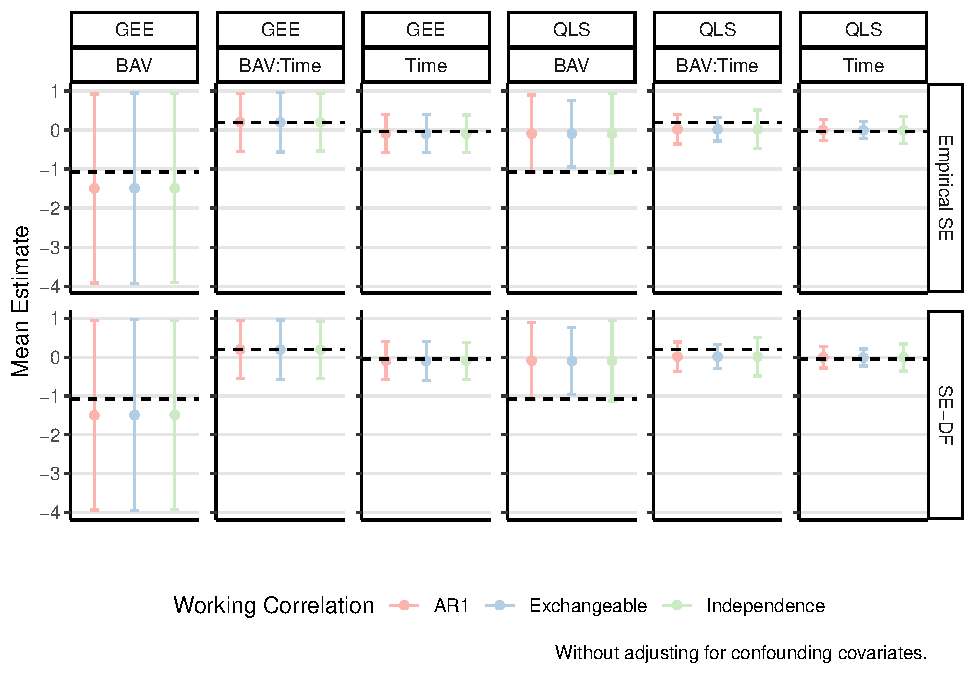
\includegraphics{FinalReport_files/figure-pdf/unnamed-chunk-6-1.pdf}

}

\caption{Comparison of Estimation Results From 1,500 Simulation}

\end{figure}%

The relative bias of estimates for the effect of BAV across different
working correlation structures (AR1, Exchangeable, Independence) using
the GEE and QLS methods, with and without including confounding
covariates, are presented in Figure 2. The dashed horizontal line at
\(y = 0\) is used as a reference to indicate 0 relative bias for
estimating the BAV effect. The left panel shows the GEE method, in which
the median relative bias values are close to zero across all correlation
structures, although considerable variability and numerous outliers
exist. In contrast, the QLS method on the right maintains consistently
low variability but a systematic positive bias in the estimates. There
is no significant difference between plots with and without inclusion of
confounding covariates. The detailed number of outliers are reported in
Appendix B.

\begin{figure}[H]

{\centering 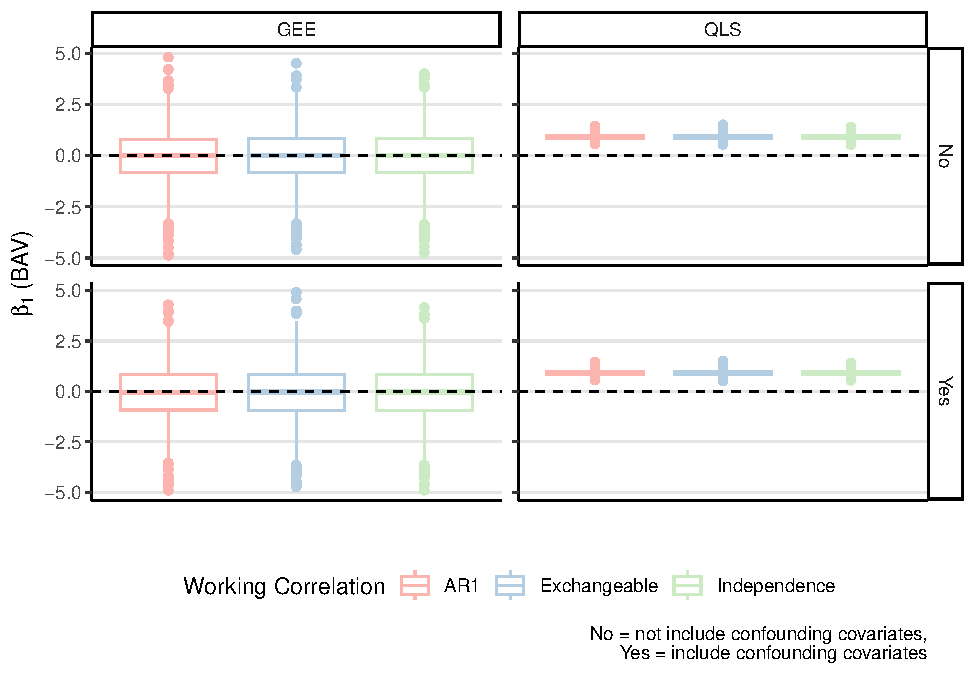
\includegraphics{FinalReport_files/figure-pdf/unnamed-chunk-7-1.pdf}

}

\caption{Relative bias of estimations for the effect of BAV using GEE
and QLS with independence, AR1, and exchangeable working correlation
structures.}

\end{figure}%

Figure 3 illustrates the relative bias in the coefficient estimates of
the interaction effect between BAV and time. With the same layout as
Figure 2, the GEE method provides nearly unbiased estimates of
\(\beta_3\) on average but exhibits significant variability. In
contrast, the QLS method produces negatively biased estimates with low
variability.

\begin{figure}[H]

{\centering 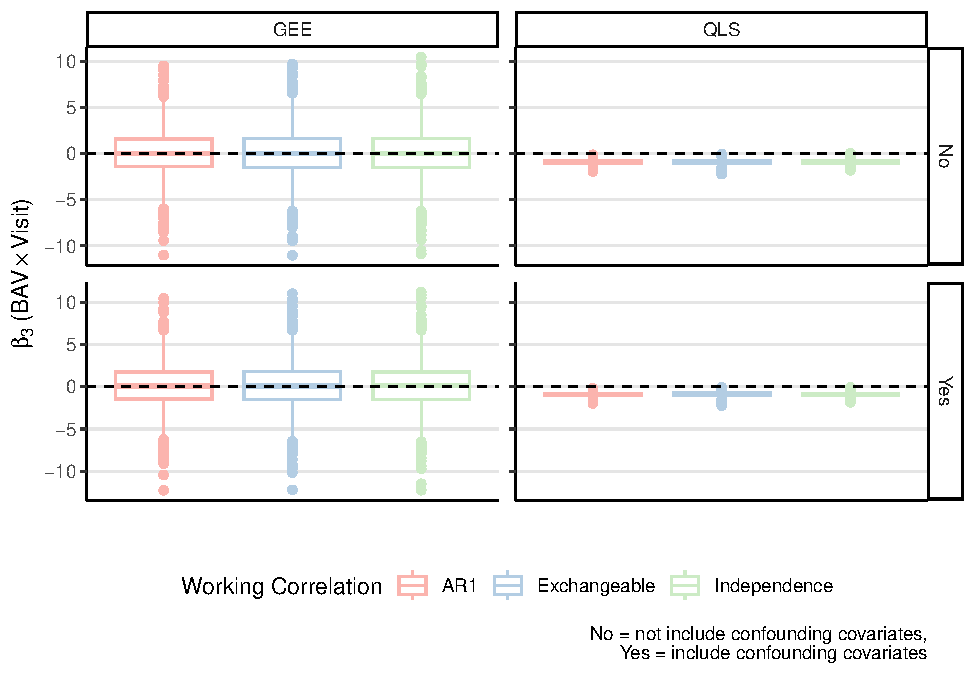
\includegraphics{FinalReport_files/figure-pdf/unnamed-chunk-8-1.pdf}

}

\caption{Relative bias of estimations for the interaction effect of BAV
and time using GEE and QLS with independence, AR1, and exchangeable
working correlation structures.}

\end{figure}%

The comparison of the mean estimation for correlations \(\alpha\) among
longitudinal measurements between GEE and QLS methods is shown in Table
2. As indicated by the column truth, the true correlation is set to be
0.3 at the simulation stage. When the working correlation is correctly
specified, i.e., AR1, the GEE method exhibits a mean estimate of 0.236
with a bias of -0.064 when no covariate set is considered, and a mean
estimate of 0.185 with a bias of -0.115 when covariates are included.
The QLS method shows a mean estimate of 0.725 with a bias of 0.425,
irrespective of covariate inclusion. On the other hand, when the working
correlation is misspecified to be exchangeable, the GEE method yields a
mean estimate of 0.124 with a bias of -0.176 without covariates, and a
mean estimate of 0.086 with a bias of -0.214 with covariates. Meanwhile,
the QLS method provides mean estimates of 0.560 and 0.723, with
corresponding biases of 0.260 and 0.423, respectively.

\begin{table}[H]
\centering\centering
\caption{\footnotesize Comparison of mean estimation for the correlation among longitudinal measurements using GEE and QLS methods, with and without adjustment for age, sex, and BSA.}
\centering
\resizebox{\ifdim\width>\linewidth\linewidth\else\width\fi}{!}{
\fontsize{8}{10}\selectfont
\begin{tabular}[t]{>{}llrrrrr}
\toprule
\multicolumn{3}{c}{ } & \multicolumn{2}{c}{GEE} & \multicolumn{2}{c}{QLS} \\
\cmidrule(l{3pt}r{3pt}){4-5} \cmidrule(l{3pt}r{3pt}){6-7}
Working Correlation & Covariate Set & Truth & Mean Estimate & Bias & Mean Estimate & Bias\\
\midrule
 & No & 0.3 & 0.236 & -0.064 & 0.725 & 0.425\\
\cmidrule{2-7}
\multirow[t]{-2}{*}{\raggedright\arraybackslash \textbf{AR1}} & Yes & 0.3 & 0.185 & -0.115 & 0.723 & 0.423\\
\cmidrule{1-7}
 & No & 0.3 & 0.124 & -0.176 & 0.560 & 0.260\\
\cmidrule{2-7}
\multirow[t]{-2}{*}{\raggedright\arraybackslash \textbf{Exchangeable}} & Yes & 0.3 & 0.086 & -0.214 & 0.723 & 0.423\\
\bottomrule
\multicolumn{7}{l}{\rule{0pt}{1em}\textsuperscript{*} Covariate Set: Yes = Included confounding covariates, No = Without confounding covariates}\\
\end{tabular}}
\end{table}

Table 3 presents the estimation of correlations (\(\tau\)) between
subjects in matched pairs using the QLS approach, across the three
different working correlations and covariate sets (with and without
confounder adjustment). In general, the differences in the intra-pair
correlation estimation between models with and without confounding
covariates are ignorable irrespective of the specified working
correlation. When the specified working correlation matches with the
true working correlation (AR1), he intra-pair correlation is estimated
to be the lowest, at around 0.362, similar to the estimate based on
exchangeable working correlation. However, the intra-pair correlation is
estimated to around 0.5 when the working correlation is specified to be
independence.

\begin{table}[H]
\centering\centering
\caption{\footnotesize Estimation of correlations between subjects in matched pairs using QLS approach.}
\centering
\resizebox{\ifdim\width>\linewidth\linewidth\else\width\fi}{!}{
\fontsize{8}{10}\selectfont
\begin{tabular}[t]{>{}lrrrr}
\toprule
\multicolumn{1}{c}{ } & \multicolumn{2}{c}{No Confounders} & \multicolumn{2}{c}{With Confounders} \\
\cmidrule(l{3pt}r{3pt}){2-3} \cmidrule(l{3pt}r{3pt}){4-5}
Working Correlation & Mean $\tau$ & SD $\tau$ & Mean $\tau$ & SD $\tau$\\
\midrule
\textbf{AR1} & 0.362 & 0.143 & 0.362 & 0.143\\
\textbf{Exchangeable} & 0.390 & 0.114 & 0.391 & 0.114\\
\textbf{Independence} & 0.484 & 0.093 & 0.486 & 0.093\\
\bottomrule
\end{tabular}}
\end{table}

\begin{figure}[H]

{\centering 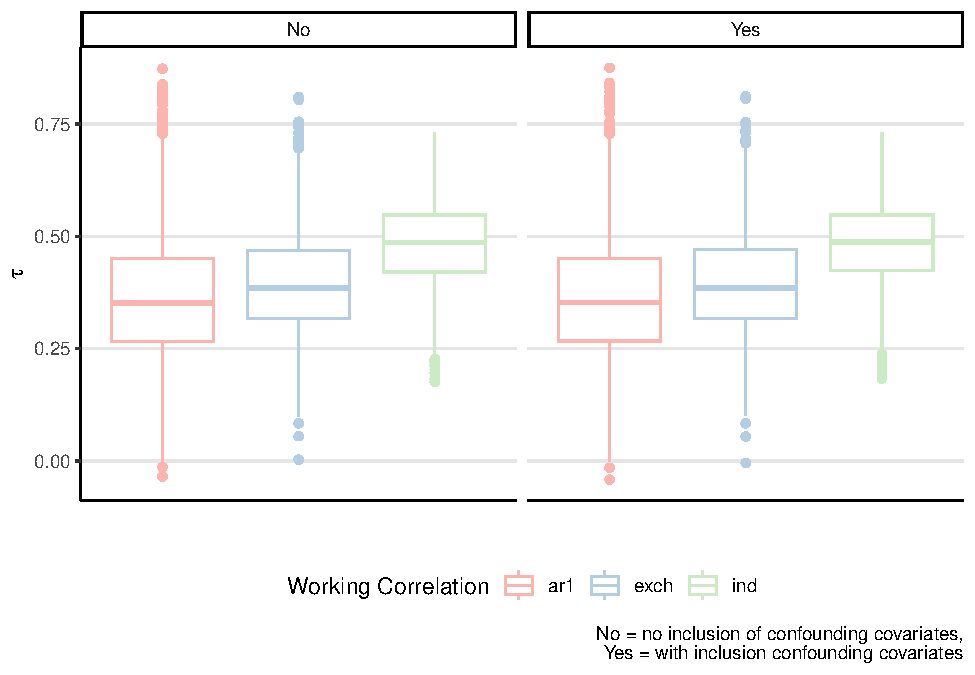
\includegraphics[width=0.7\textwidth,height=\textheight]{FinalReport_files/figure-pdf/unnamed-chunk-12-1.pdf}

}

\caption{Estimation of intra-pair correlation using QLS approach across
three different working correlation structures for both with and without
inclusion of confounding covariates.}

\end{figure}%

\section{Discusssion}\label{discusssion}

In this study, we compared the performance of the GEE and QLS methods in
modelling binary outcomes of aortic root diameter in patients with
bicuspid aortic valves (BAV) versus tricuspid aortic valves (TAV). Both
methods were evaluated across different working correlation structures.
Our findings indicate that, within this small sample context (20 to 25
matched pairs), the GEE method shows considerable variability in its
estimates, whereas the QLS method, although more consistent, exhibits
systematic positive bias. The choice of working correlation structure
significantly impacts the parameter estimates. The AR1 structure
provided more accurate estimates in GEE because it aligns with the true
working correlation used in simulating the data.

In our simulation study, we noticed that the GEE method tended to be
unstable with small sample sizes, leading to variability in the
estimates. On the other hand, the QLS method provided more consistent
results, but these were often biased. This means that QLS might either
underestimate or overestimate the true effects because of how it deals
with the correlation structure. Interestingly, even though we tested
different working correlation structures (AR1, exchangeable, and
independence), the parameter estimates for each method didn't change
much. This suggests that for small matched samples, the specific choice
of correlation structure might not significantly affect the overall
estimates for binary outcomes. However, it's still crucial to choose the
right correlation structure to ensure accurate standard errors and
confidence intervals.

In the clinical context of aortic root diameter changes in BAV patients
post-surgery, the methodological differences between GEE and QLS can
influence clinical decision-making. Accurate modelling of aortic root
changes is crucial for assessing the risk of aortic dilatation and
planning follow-up care. As shown in Figure 1, the true effect of BAV is
estimated to be around -1. However, the QLS method provides an average
estimate of around 0, indicating a substantial positive bias. As a
comparison, although with more variability, the GEE method offers more
conservative and closer-to-true estimates for the effect of BAV and its
interaction with time. These estimation differences can have important
implications for clinical decisions. Overestimating the effect of
interventions or conditions like BAV due to biased estimates from QLS
may lead to inappropriate clinical strategies. On the other hand, the
variability in GEE estimates requires careful interpretation to avoid
misjudging the treatment effect.

It's important to note several limitations. While using simulated data
allows for controlled studies, it might not fully reflect the
complexities of real-world data. Both GEE and QLS methods have
limitations in handling informative dropouts and covariate endogeneity,
which could affect the robustness of the estimates. The small sample
size poses challenges for the GEE method, potentially leading to
underestimated standard errors and variability in estimates. The
informative dropout process modelled in our simulations may not fully
capture real-world complexities. However, it also presents an
opportunity for further investigations to refine GEE and QLS approaches
for handling informative dropouts and covariate endogeneity in
longitudinal studies.

In conclusion, our comparative analysis of GEE and QLS methods
underscores the importance of methodological considerations in
longitudinal data analysis. While GEE showed a better ability to capture
the correlation among repeated measurements, QLS demonstrated lower
variability and consistent parameter estimates across different
correlation structures. These robust findings offer confident guidance
for researchers in selecting appropriate analytical approaches for their
studies, reinforcing the importance of methodological considerations in
longitudinal data analysis.

\newpage

\section{Appendix A}\label{appendix-a}

\subsection{\texorpdfstring{Estimation for Stage One
\(\alpha\)}{Estimation for Stage One \textbackslash alpha}}\label{estimation-for-stage-one-alpha}

Since the maximum number repeated measurement within the same subject is
restricted to 6, we take \(t_{ij} = 4\) as an example for simplicity.
The intravisit correlation structure is \[
R_i(\alpha) = 
\begin{bmatrix}
1 & \alpha & \alpha^2 & \alpha^3\\
\alpha & 1 & \alpha & \alpha^2\\
\alpha^2 & \alpha & 1 & \alpha\\
\alpha^3 & \alpha^2 & \alpha & 1
\end{bmatrix}
\] The partial derivative of covariance matrix with respect to
\(\alpha\) is \[
\frac{\partial F_i^{-1}(\alpha)}{\partial \alpha} = \frac{\partial{R_i^{-1}(\alpha)}}{\partial \alpha} \otimes Q_i^{-1}(\tau)
\] because \(Q^{-1}_i(\tau)\) does not contain \(\alpha\). \[
\frac{\partial{R_i^{-1}(\alpha)}}{\partial \alpha} = -R_i^{-1}(\alpha) \frac{\partial R_i(\alpha)}{\partial \alpha} R_i^{-1}(\alpha)
\]

\[
\frac{\partial R_i(\alpha)}{\partial \alpha}= 
\begin{bmatrix}
0 & 1 & 2\alpha & 3\alpha^2\\
1 & 0 & 1 & 2\alpha\\
2\alpha & 1 & 0 & 1\\
3\alpha^2 & 2\alpha & 1 & 0
\end{bmatrix}
\] Therefore, \[
\frac{\partial{R_i^{-1}(\alpha)}}{\partial \alpha}= 
\frac{1}{(1-\alpha^2)^2}
\begin{bmatrix}
2\alpha & -(1+\alpha^2) & 0 & 0\\
-(1+\alpha^2) & 4\alpha & -(1+\alpha^2) & 0\\
0 & -(1+\alpha^2) & 4\alpha & -(1+\alpha^2)\\
0 & 0 & -(1+\alpha^2) & 0
\end{bmatrix}
\] \[
\frac{\partial{R_i^{-1}(\alpha)}}{\partial \alpha}\otimes Q_i^{-1} = 
\frac{1}{(1-\alpha^2)^2}
\begin{bmatrix}
2\alpha Q_i^{-1} & -(1+\alpha^2) Q_i^{-1} & 0 & 0\\
-(1+\alpha^2) Q_i^{-1} & 4\alpha Q_i^{-1} & -(1+\alpha^2) Q_i^{-1} & 0\\
0 & -(1+\alpha^2) Q_i^{-1} & 4\alpha Q_i^{-1} & -(1+\alpha^2) Q_i^{-1}\\
0 & 0 & -(1+\alpha^2) Q_i^{-1} & 2\alpha Q_i^{-1}
\end{bmatrix}
\] Hence, \[
\begin{aligned}
\frac{\partial Q(\beta, \Gamma)}{\partial \alpha} &= 
\sum_{i=1}^m \sum_{j=1}^2 
\begin{pmatrix}
Z_{i1} & Z_{i2} & Z_{i3} & Z_{i4} 
\end{pmatrix}
\frac{\partial{R_i^{-1}(\alpha)}}{\partial \alpha}\otimes Q_i^{-1}
\begin{pmatrix}
Z_{i1} \\ Z_{i2} \\ Z_{i3} \\ Z_{i4} 
\end{pmatrix}\\
&= \frac{1}{(1-\alpha^2)^2} \sum_{i=1}^m \sum_{j=1}^2 
\Big\{2\alpha \Big(Z_{ij1}Q_i^{-1}Z_{ij1} + 2Z_{ij2}Q_i^{-1}Z_{ij2}+  2Z_{ij3}Q_i^{-1}Z_{ij3}+Z_{ij4}Q_i^{-1}Z_{ij4}\Big)\\
& \quad \quad \quad \quad \quad\quad 2(1+\alpha^2)\cdot 
\Big(Z_{ij1}Q_i^{-1}Z_{ij2}+Z_{ij2}Q_i^{-1}Z_{ij3}+Z_{ij3}Q_i^{-1}Z_{ij4}\Big)
\Big\}\\
&= \sum_{i=1}^m \sum_{j=1}^2 \left\{\alpha 
\left(\sum_{k=1}^{t_{ij}} Z_{ijk}'Q_i^{-1} Z_{ijk} + \sum_{k=2}^{t_{ij} - 1}Z_{ijk}'Q_i^{-1} Z_{ijk}\right) - (1+\alpha^2)\left(\sum_{k=1}^{t_{ij} - 1}Z_{ijk}'Q_i^{-1}Z_{ijk+1}\right) \right\}
\end{aligned}
\] Let
\(S_1 = \sum_{k=1}^{t_{ij}} Z_{ijk}'Q_i^{-1} Z_{ijk} + \sum_{k=2}^{t_{ij} - 1}Z_{ijk}'Q_i^{-1} Z_{ijk}\)
and \(S_2 = \sum_{k=1}^{t_{ij} - 1}Z_{ijk}'Q_i^{-1}Z_{ijk+1}\), then \[
\begin{aligned}
\frac{\partial Q(\beta, \Gamma)}{\partial \alpha} &= \sum_{i=1}^m \sum_{j=1}^2 \big(\alpha S_1 - (1+\alpha^2) S_2\big) \\
&= \sum_{i=1}^m \sum_{j=1}^2\big(\alpha S_1 - S_2-\alpha^2S_2\big) = 0\\
& \sum_{i=1}^m \sum_{j=1}^2\big(\alpha^2 S_2 -\alpha S_1 + S_2\big) = 0\\
\hat{\alpha}_0 &= \sum_{i=1}^m \sum_{j=1}^2\frac{S_1+\sqrt{S_1^2+4S_2^2}}{2S_2}
\end{aligned}
\]

\newpage

\section{Appendix B}\label{appendix-b}

\subsection{Coverage Probability}\label{coverage-probability}

\begin{table}[!h]
\centering\centering
\caption{\footnotesize The Coverage Probability of Regression Coefficient Estimation from GEE and QLS.}
\centering
\resizebox{\ifdim\width>\linewidth\linewidth\else\width\fi}{!}{
\fontsize{8}{10}\selectfont
\begin{tabular}[t]{lrrrrrrrrl}
\toprule
\multicolumn{2}{c}{ } & \multicolumn{4}{c}{GEE} & \multicolumn{4}{c}{QLS} \\
\cmidrule(l{3pt}r{3pt}){3-6} \cmidrule(l{3pt}r{3pt}){7-10}
\multicolumn{2}{c}{ } & \multicolumn{2}{c}{No Confounders} & \multicolumn{2}{c}{With Confounders} & \multicolumn{2}{c}{No Confounders} & \multicolumn{2}{c}{With Confounders} \\
\cmidrule(l{3pt}r{3pt}){3-4} \cmidrule(l{3pt}r{3pt}){5-6} \cmidrule(l{3pt}r{3pt}){7-8} \cmidrule(l{3pt}r{3pt}){9-10}
Corstr & Term & Empirical SE & DF-SE & Empirical SE & DF-SE & Empirical SE & DF-SE & Empirical SE & DF-SE\\
\midrule
(Intercept) & 0.880 & 0.893 & 0.917 & 0.920 & 0.000 & 0.000 & 1.000 & 1.000 & Independence\\
bav & 0.903 & 0.909 & 0.906 & 0.909 & 0.527 & 0.547 & 0.534 & 0.564 & Independence\\
bav:visit & 0.853 & 0.857 & 0.856 & 0.859 & 1.000 & 1.000 & 1.000 & 1.000 & Independence\\
visit & 0.881 & 0.888 & 0.887 & 0.890 & 1.000 & 1.000 & 1.000 & 1.000 & Independence\\
(Intercept) & 0.881 & 0.891 & 0.922 & 0.925 & 0.001 & 0.001 & 0.968 & 0.970 & AR1\\
\addlinespace
bav & 0.911 & 0.918 & 0.913 & 0.917 & 0.484 & 0.497 & 0.492 & 0.517 & AR1\\
bav:visit & 0.867 & 0.876 & 0.879 & 0.883 & 0.979 & 0.979 & 0.981 & 0.983 & AR1\\
visit & 0.898 & 0.906 & 0.907 & 0.909 & 1.000 & 1.000 & 1.000 & 1.000 & AR1\\
(Intercept) & 0.882 & 0.892 & 0.914 & 0.915 & 0.000 & 0.000 & 0.936 & 0.940 & Exchangeable\\
bav & 0.904 & 0.911 & 0.909 & 0.910 & 0.277 & 0.290 & 0.287 & 0.308 & Exchangeable\\
\addlinespace
bav:visit & 0.856 & 0.862 & 0.866 & 0.870 & 0.899 & 0.903 & 0.906 & 0.917 & Exchangeable\\
visit & 0.874 & 0.881 & 0.879 & 0.883 & 1.000 & 1.000 & 1.000 & 1.000 & Exchangeable\\
\bottomrule
\end{tabular}}
\end{table}

\subsection{Simulation Results}\label{simulation-results-1}

\begin{table}[!h]
\centering\centering\begingroup\fontsize{8}{10}\selectfont

\resizebox{\ifdim\width>\linewidth\linewidth\else\width\fi}{!}{
\begin{tabular}{>{}lllrrrrrr}
\toprule
Corstr & Type & Term & True Value & Mean Est & SD Est & Mean SE & Mean SE-DF & Mean MSE\\
\midrule
 &  & Intercept & -1.784 & -1.937 & 3.702 & 2.795 & 2.853 & 13.731\\
\cmidrule{3-9}
 &  & BAV & -1.077 & -1.541 & 4.088 & 1.276 & 1.303 & 16.924\\
\cmidrule{3-9}
 &  & BAV:Visit & 0.192 & 0.209 & 0.527 & 0.397 & 0.405 & 0.278\\
\cmidrule{3-9}
 & \multirow[t]{-4}{*}{\raggedright\arraybackslash GEE} & Visit & -0.042 & -0.085 & 0.330 & 0.258 & 0.263 & 0.111\\
\cmidrule{2-9}
 &  & Intercept & -1.784 & 0.137 & 0.319 & 2.008 & 2.051 & 3.791\\
\cmidrule{3-9}
 &  & BAV & -1.077 & -0.091 & 0.117 & 0.507 & 0.517 & 0.986\\
\cmidrule{3-9}
 &  & BAV:Visit & 0.192 & 0.016 & 0.044 & 0.192 & 0.196 & 0.033\\
\cmidrule{3-9}
\multirow[t]{-8}{*}[1\dimexpr\aboverulesep+\belowrulesep+\cmidrulewidth]{\raggedright\arraybackslash \textbf{AR1}} & \multirow[t]{-4}{*}{\raggedright\arraybackslash QLS} & Visit & -0.042 & -0.004 & 0.032 & 0.140 & 0.143 & 0.002\\
\bottomrule
\multicolumn{9}{l}{\rule{0pt}{1em}\textit{Corstr: } \textsuperscript{*} Correlation Structure}\\
\end{tabular}}
\endgroup{}
\end{table}

\begin{table}[!h]
\centering\centering\begingroup\fontsize{8}{10}\selectfont

\resizebox{\ifdim\width>\linewidth\linewidth\else\width\fi}{!}{
\begin{tabular}{>{}lllrrrrrr}
\toprule
Corstr & Type & Term & True Value & Mean Est & SD Est & Mean SE & Mean SE-DF & Mean MSE\\
\midrule
 &  & Intercept & -1.784 & -1.931 & 3.726 & 2.805 & 2.863 & 13.901\\
\cmidrule{3-9}
 &  & BAV & -1.077 & -1.540 & 4.102 & 1.283 & 1.309 & 17.040\\
\cmidrule{3-9}
 &  & BAV:Visit & 0.192 & 0.208 & 0.547 & 0.401 & 0.409 & 0.300\\
\cmidrule{3-9}
 & \multirow[t]{-4}{*}{\raggedright\arraybackslash GEE} & Visit & -0.042 & -0.092 & 0.338 & 0.260 & 0.265 & 0.116\\
\cmidrule{2-9}
 &  & Intercept & -1.784 & 0.139 & 0.314 & 1.702 & 1.739 & 3.797\\
\cmidrule{3-9}
 &  & BAV & -1.077 & -0.093 & 0.117 & 0.438 & 0.447 & 0.981\\
\cmidrule{3-9}
 &  & BAV:Visit & 0.192 & 0.018 & 0.043 & 0.155 & 0.159 & 0.032\\
\cmidrule{3-9}
\multirow[t]{-8}{*}[1\dimexpr\aboverulesep+\belowrulesep+\cmidrulewidth]{\raggedright\arraybackslash \textbf{Exchangeable}} & \multirow[t]{-4}{*}{\raggedright\arraybackslash QLS} & Visit & -0.042 & -0.006 & 0.032 & 0.112 & 0.115 & 0.002\\
\bottomrule
\multicolumn{9}{l}{\rule{0pt}{1em}\textit{Corstr:} \textsuperscript{*} Correlation Structure}\\
\end{tabular}}
\endgroup{}
\end{table}

\begin{table}[!h]
\centering\centering\begingroup\fontsize{8}{10}\selectfont

\resizebox{\ifdim\width>\linewidth\linewidth\else\width\fi}{!}{
\begin{tabular}{>{}lllrrrrrr}
\toprule
Corstr & Type & Term & True Value & Mean Est & SD Est & Mean SE & Mean SE-DF & Mean MSE\\
\midrule
 &  & Intercept & -1.784 & -1.903 & 3.700 & 2.795 & 2.853 & 13.703\\
\cmidrule{3-9}
 &  & BAV & -1.077 & -1.540 & 4.103 & 1.280 & 1.307 & 17.047\\
\cmidrule{3-9}
 &  & BAV:Visit & 0.192 & 0.207 & 0.546 & 0.394 & 0.402 & 0.298\\
\cmidrule{3-9}
 & \multirow[t]{-4}{*}{\raggedright\arraybackslash GEE} & Visit & -0.042 & -0.090 & 0.337 & 0.256 & 0.261 & 0.116\\
\cmidrule{2-9}
 &  & Intercept & -1.784 & 0.138 & 0.315 & 2.755 & 2.814 & 3.793\\
\cmidrule{3-9}
 &  & BAV & -1.077 & -0.092 & 0.114 & 0.525 & 0.536 & 0.983\\
\cmidrule{3-9}
 &  & BAV:Visit & 0.192 & 0.017 & 0.040 & 0.247 & 0.252 & 0.032\\
\cmidrule{3-9}
\multirow[t]{-8}{*}[1\dimexpr\aboverulesep+\belowrulesep+\cmidrulewidth]{\raggedright\arraybackslash \textbf{Independence}} & \multirow[t]{-4}{*}{\raggedright\arraybackslash QLS} & Visit & -0.042 & -0.004 & 0.029 & 0.173 & 0.176 & 0.002\\
\bottomrule
\multicolumn{9}{l}{\rule{0pt}{1em}\textit{Corstr, SD, MSE: } \textsuperscript{*} Correlation Structure, Standard Deviation and Mean Squared Error}\\
\end{tabular}}
\endgroup{}
\end{table}

\subsection{Outliers in Relative Bias}\label{outliers-in-relative-bias}

\textbf{BAV}

\begin{table}[H]
\centering\centering
\caption{Outliers in Relative Bias for the effect of BAV}
\centering
\begin{tabular}[t]{lllr}
\toprule
Method & Working Correlation & Confounders & No.Outliers\\
\midrule
 & Exchangeable & No & 16\\
\cmidrule{2-4}
 & Independence & No & 16\\
\cmidrule{2-4}
 &  & Yes & 17\\
\cmidrule{3-4}
 & \multirow[t]{-2}{*}{\raggedright\arraybackslash AR1} & No & 18\\
\cmidrule{2-4}
 & Independence & Yes & 18\\
\cmidrule{2-4}
\multirow[t]{-6}{*}[4\dimexpr\aboverulesep+\belowrulesep+\cmidrulewidth]{\raggedright\arraybackslash QLS} & Exchangeable & Yes & 20\\
\cmidrule{1-4}
 & AR1 & Yes & 36\\
\cmidrule{2-4}
 &  & No & 37\\
\cmidrule{3-4}
 & \multirow[t]{-2}{*}{\raggedright\arraybackslash Exchangeable} & Yes & 39\\
\cmidrule{2-4}
 &  & No & 40\\
\cmidrule{3-4}
 & \multirow[t]{-2}{*}{\raggedright\arraybackslash Independence} & Yes & 40\\
\cmidrule{2-4}
\multirow[t]{-6}{*}[3\dimexpr\aboverulesep+\belowrulesep+\cmidrulewidth]{\raggedright\arraybackslash GEE} & AR1 & No & 42\\
\bottomrule
\end{tabular}
\end{table}

\textbf{Time}

\begin{table}[H]
\centering\centering
\caption{Outliers in Relative Bias for the effect of Time}
\centering
\begin{tabular}[t]{lllr}
\toprule
Method & Working Correlation & Confounders & No.Outliers\\
\midrule
 &  & No & 12\\
\cmidrule{3-4}
 & \multirow[t]{-2}{*}{\raggedright\arraybackslash AR1} & Yes & 13\\
\cmidrule{2-4}
 &  & Yes & 15\\
\cmidrule{3-4}
 & \multirow[t]{-2}{*}{\raggedright\arraybackslash Exchangeable} & No & 16\\
\cmidrule{2-4}
 &  & Yes & 21\\
\cmidrule{3-4}
\multirow[t]{-6}{*}[2\dimexpr\aboverulesep+\belowrulesep+\cmidrulewidth]{\raggedright\arraybackslash QLS} & \multirow[t]{-2}{*}{\raggedright\arraybackslash Independence} & No & 27\\
\cmidrule{1-4}
 &  & No & 41\\
\cmidrule{3-4}
 & \multirow[t]{-2}{*}{\raggedright\arraybackslash AR1} & Yes & 41\\
\cmidrule{2-4}
 & Exchangeable & No & 42\\
\cmidrule{2-4}
 & Independence & Yes & 43\\
\cmidrule{2-4}
 & Exchangeable & Yes & 44\\
\cmidrule{2-4}
\multirow[t]{-6}{*}[4\dimexpr\aboverulesep+\belowrulesep+\cmidrulewidth]{\raggedright\arraybackslash GEE} & Independence & No & 44\\
\bottomrule
\end{tabular}
\end{table}

\textbf{Interaction Effect between BAV and Time}

\begin{table}[H]
\centering\centering
\caption{Outliers in Relative Bias for the interaction effect between BAV and Time}
\centering
\begin{tabular}[t]{lllr}
\toprule
Method & Working Correlation & Confounders & No.Outliers\\
\midrule
 &  & No & 12\\
\cmidrule{3-4}
 & \multirow[t]{-2}{*}{\raggedright\arraybackslash Exchangeable} & Yes & 14\\
\cmidrule{2-4}
 &  & No & 23\\
\cmidrule{3-4}
 & \multirow[t]{-2}{*}{\raggedright\arraybackslash AR1} & Yes & 23\\
\cmidrule{2-4}
 &  & Yes & 29\\
\cmidrule{3-4}
\multirow[t]{-6}{*}[2\dimexpr\aboverulesep+\belowrulesep+\cmidrulewidth]{\raggedright\arraybackslash QLS} & \multirow[t]{-2}{*}{\raggedright\arraybackslash Independence} & No & 30\\
\cmidrule{1-4}
 &  & No & 40\\
\cmidrule{3-4}
 & \multirow[t]{-2}{*}{\raggedright\arraybackslash AR1} & Yes & 41\\
\cmidrule{2-4}
 & Exchangeable & Yes & 44\\
\cmidrule{2-4}
 & Independence & Yes & 44\\
\cmidrule{2-4}
 & Exchangeable & No & 45\\
\cmidrule{2-4}
\multirow[t]{-6}{*}[4\dimexpr\aboverulesep+\belowrulesep+\cmidrulewidth]{\raggedright\arraybackslash GEE} & Independence & No & 45\\
\bottomrule
\end{tabular}
\end{table}

\newpage

\section{Appendix C: Code}\label{appendix-c-code}

\subsection{Full Data Simulation}\label{full-data-simulation-1}

\begin{verbatim}
# Required R packages ---------------------------------------------
library(CorBin)
library(tidyverse)
library(geepack)
library(parallel)
library(survival)
library(simsurv)
library(doParallel)

load("data/realcoefs.RData")

# Set up parallel backend
num_cores <- detectCores() - 1  # Use one less core than available
cl <- makeCluster(num_cores)
registerDoParallel(cl)

# Global Variables ------------------------------------------------
n_patients <- 250 
n_sim <- 1500
maxT <- 6
rho <- 0.3
alpha_ci <- 0.05

true_coefs <- red_ar1$coefficients$Estimate
names(true_coefs) <- c("g0", "bav", "visit", "bav_visit")
corr_alpha <- red_ar1$corr$Estimate
surv_coefs <- surv_coefs[,-4]
rownames(surv_coefs)[4] <- "male"

# Helper Functions -------------------------------------------------
# 1. Function for creating profile for one simulation 
patient_profile <- function(){
  
  full_data <- NULL 
  
  for (id in 1:n_patients){
    # Simulate covariates
    age = rnorm(1, mean = 50, sd = 10)
    male = rbinom(1, size = 1, prob = 0.65)
    bsa = rnorm(1, mean = 2, sd = 0.3)
    logit_bav <- ps_coefs[1] + ps_coefs[2]*age + 
                 ps_coefs[3]*male + ps_coefs[4]*bsa
    prob_bav <- exp(logit_bav) / (1+exp(logit_bav))
    bav = rbinom(1, size = 1, prob = prob_bav)
    
    # Simulate binary outcome 
    vst <- 1:maxT
    logit_y <- true_coefs[1] + true_coefs[2]*bav + 
               true_coefs[3]*vst + true_coefs[4]*bav*vst
    prob_y <- exp(logit_y) / (1+exp(logit_y)) 
    y <- t(cBern(n = 1, p = prob_y, rho = rho, type = "DCP"))
    
    full_data <- rbind(full_data, 
                       data.frame(id = rep(id, each = maxT), 
                                  age = rep(age, each = maxT), 
                                  male = rep(male, each = maxT), 
                                  bsa = rep(bsa, each = maxT), 
                                  bav = rep(bav, each = maxT), 
                                  visit = vst, 
                                  total_visit = maxT) %>% cbind(y)
    )
  }
  
  full_data
}

# 2. Function to simulate dropouts 
sim_dropouts <- function(dat){
  
  temp <- dat %>% relocate(c(y, bav), .after = id) 
  
  base_df <- temp %>% filter(visit == 1) %>% select(-visit, -total_visit)
  
  # (1) Drop visits for patients who had only one follow up 
  pat_set1 <- simsurv(lambdas = exp(surv_coefs$fit1[6]), # scale parameter
                      gammas = exp(surv_coefs$fit1[7]), # shape parameter
                      x = base_df, maxt = 1, 
                      betas = t(surv_coefs)[1,1:5],
                      dist = "weibull") %>% 
                      filter(status == 1) %>% pull(id)
  temp <- temp %>% 
    filter(!((id %in% pat_set1) & visit > 2)) %>% 
    group_by(id) %>% 
    mutate(total_visit = n()) %>% 
    ungroup()
  
  
  # (2) Drop visits for patients who had two follow up visits, 
  #     i.e., total_visit == 3 
  Z2 <- temp %>% filter(total_visit > 2) %>% 
    group_by(id) %>% slice(1) %>% 
    select(-c(visit, total_visit))
  pat_set2 <- simsurv(lambdas = exp(surv_coefs$fit2[6]), # scale parameter
                      gammas = exp(surv_coefs$fit2[7]), # shape parameter
                      x = Z2, maxt = 1, 
                      betas = t(surv_coefs)[2,1:5],
                      dist = "weibull") %>% 
                      filter(status == 1)  %>% pull(id)
  temp <- temp %>% 
    filter(!((id %in% pat_set2) & visit > 3)) %>% 
    group_by(id) %>% 
    mutate(total_visit = n()) %>% 
    ungroup()
  
  # (3) Drop visits for patients who had three follow up visits, 
  #     i.e., total_visit == 4 
  Z3 <- temp %>% group_by(id) %>% slice(1) %>% 
    filter(total_visit > 3) %>% select(-c(visit, total_visit))
  pat_set3 <- simsurv(lambdas = exp(surv_coefs$fit3[6]), 
                      gammas = exp(surv_coefs$fit3[7]), # shape parameter
                      x = Z3, maxt = 1,
                      betas = t(surv_coefs)[3,1:5],
                      dist = "weibull") %>% 
                      filter(status == 1) %>% pull(id)
  temp <- temp %>% 
    filter(!((id %in% pat_set3) & visit > 4)) %>% 
    group_by(id) %>% 
    mutate(total_visit = n()) %>% 
    ungroup()
  
  # (4) Drop visits for patients who had four follow up visits, 
  #     i.e., total_visit == 5 
  Z4 <- temp %>% group_by(id) %>% slice(1)%>% 
    filter(total_visit == 6)  %>% select(-c(visit, total_visit))
  pat_set4 <- simsurv(lambdas = exp(surv_coefs$fit5[6]), 
                      gammas = exp(surv_coefs$fit5[7]), # shape parameter
                      x = Z4, maxt = 1,
                      betas = t(surv_coefs)[4,1:5],
                      dist = "weibull") %>% 
                      filter(status == 1)  %>% pull(id)
  temp <- temp %>% 
    filter(!((id %in% pat_set4) & visit > 5)) %>% 
    # filter(!((id %in% Z4$id[pat_set4]) & visit > 5)) %>% 
    group_by(id) %>% 
    mutate(total_visit = n()) %>% 
    ungroup()
  
  temp 
}


set.seed(5207)
sim_df <- expand.grid(sim_id = 1:n_sim) %>%
  mutate(full_data= map(sim_id, function(id){patient_profile()})) %>%
  mutate(dropout_data = map(full_data, ~sim_dropouts(.x))) 

# Stop the parallel backend
stopCluster(cl)
\end{verbatim}

\subsection{Propensity Score Matching}\label{propensity-score-matching}

\begin{verbatim}
library(optmatch)
library(tidyverse)
library(lme4)

ps_match <- function(dat){
  base_info <- dat %>% filter(visit == 1) %>% select(-total_visit)
  ps_model <- glm(bav ~ age + male + bsa, 
                  family = binomial, data = base_info)
  pps_match <- pairmatch(ps_model, data = base_info)
  matched_df <- data.frame(base_info, matched = pps_match, 
                           check.rows = TRUE) %>% 
                           filter(!is.na(matched))
  matchid <- matched_df %>% select(id, matched)
  finaldata <- dat %>% right_join(matchid, by = "id")
  finaldata
}

matched_df <- sim_df %>% 
  mutate(matched_full =  map(full_data, ~ps_match(.x))) %>% 
  mutate(matched_ddat = map(dropout_data, ~ps_match(.x))) %>% 
  matched_df %>% select(matched_full, matched_ddat)
\end{verbatim}

\newpage

\subsection{QLS Functions}\label{qls-functions}

\begin{verbatim}
# 1. Function to create exchangeable correlation matrix
exch_cormat <- function(rho, n) {
  cor_matrix <- matrix(rho, n, n)
  diag(cor_matrix) <- 1
  return(cor_matrix)
}

# 2. Function to create AR(1) correlation matrix
ar1_cormat <- function(rho, n) {
  rho <- as.numeric(rho)
  exponent <- abs(matrix(1:n - 1, nrow = n, ncol = n, 
                         byrow = TRUE) - (1:n - 1))
  return(rho^exponent)
}


# 3. Function to estimate Stage 1 tau 
tau_stg1 <- function(mdat, maxT, Z, corstr, alpha0){
  Fa <- Fb <- 0
  for (i in mdat$clusterID){
    a_1 <- a_2 <- 0
    t_i1 <- nlevels(as.factor(mdat[mdat$clusterID == i & mdat$cluster.var==1,]$visit))
    t_i2 <- nlevels(as.factor(mdat[mdat$clusterID == i & mdat$cluster.var==2,]$visit))
    if (corstr == "independence") {
      Rinv1 <- solve(diag(t_i1))
      Rinv2 <- solve(diag(t_i2))
    } 
    if (corstr == "ar1") {Rinv1 <- solve(ar1_cormat(alpha0, t_i1))} 
    if (corstr == "exchangeable") {Rinv1 <- solve(exch_cormat(alpha0, t_i1))}
    if (corstr == "ar1") {Rinv2 <- solve(ar1_cormat(alpha0, t_i2))} 
    if (corstr == "exchangeable") {Rinv2 <- solve(exch_cormat(alpha0, t_i2))}
    Rinv <- solve(exch_cormat(alpha0, maxT))
    
    Z_i1 <- Z[mdat$clusterID == i & mdat$cluster.var == 1]
    matZ_i1 <- matrix(Z_i1, nrow = t_i1)
    
    Z_i2 <- Z[mdat$clusterID == i & mdat$cluster.var == 2]
    matZ_i2 <- matrix(Z_i2, nrow = t_i2)
    
    a_1 <- a_1 + t(matZ_i1) %*% Rinv1 %*% matZ_i1 + t(matZ_i2) %*% Rinv2 %*% matZ_i2
    
    if (maxT > t_i1) {matZ_i1 <- c(matZ_i1, rep(0, maxT - t_i1))}
    if (maxT > t_i2) {matZ_i2 <- c(matZ_i2, rep(0, maxT - t_i2))}    
    
    a_2 <- a_2 + t(matZ_i1) %*% Rinv %*% matZ_i2
    
    Fa <- Fa + a_1
    Fb <- Fb + a_2
    
  }
  ### stage 1 estimate of tau
  tau0 <- ( Fa - sqrt( ( Fa - 2 * Fb ) * ( Fa + 2 * Fb ) ) ) / ( 2 * Fb )
  return(tau0)
}


# 4. Function to estimate Stage 2 tau
tau_stg2 <- function(tau0){
  tau <- as.numeric( 2 * tau0 / ( 1 + tau0 ^ 2 ) )
  return(tau)
}


# 5. Function to estimate Stage 1 alpha for AR1
alpha_stg1_ar1 <- function(mdat, Z, Qinv){
  Fa <- Fb <- 0 
  for (i in mdat$clusterID) { # for each pair
    S1_j <- S2_j <- S1_ja <- S1_jb <- 0
    
    t_i1 <- nlevels(as.factor(mdat[mdat$clusterID == i & mdat$cluster.var==1,]$visit))
    t_i2 <- nlevels(as.factor(mdat[mdat$clusterID == i & mdat$cluster.var==2,]$visit))
    t_ij <- min(c(t_i1, t_i2))
    Z_i1 <- Z[mdat$clusterID == i & mdat$cluster.var == 1]
    Z_i2 <- Z[mdat$clusterID == i & mdat$cluster.var == 2]
    
    # Check if the lengths match t_ij before creating the matrices
    if (length(Z_i1) >= t_ij && length(Z_i2) >= t_ij) {
      matZ_i1 <- matrix(Z_i1[1:t_ij], nrow = t_ij)
      matZ_i2 <- matrix(Z_i2[1:t_ij], nrow = t_ij)
      
      if (t_ij > 1) {
        for (k in 1:(t_ij-1)) {
          matZ1 <- matrix(c(matZ_i1[k], matZ_i2[k]), nrow = 2)
          matZ2 <- matrix(c(matZ_i1[k+1], matZ_i2[k+1]), nrow = 2)
          S2_j <- S2_j + t(matZ1) %*% Qinv %*% matZ2
        }
        if (t_ij == 2) {
          for (k in 1:t_ij) {
            matZ <- matrix(c(matZ_i1[k], matZ_i2[k]), nrow = 2)
            S1_j <- S1_j + t(matZ) %*% Qinv %*% matZ
          }
        } else {
          for (k in 1:t_ij) {
            matZ <- matrix(c(matZ_i1[k], matZ_i2[k]), nrow = 2)
            S1_ja <- S1_ja + t(matZ) %*% Qinv %*% matZ
          }
          for (k in 2:(t_ij-1)) {
            matZ <- matrix(c(matZ_i1[k], matZ_i2[k]), nrow = 2)
            S1_jb <- S1_jb + t(matZ) %*% Qinv %*% matZ
          }
          S1_j <- S1_ja + S1_jb
        }
      }
      
      Fa <- Fa + S1_j
      Fb <- Fb + S2_j
    } else {
      warning(paste("Cluster", i, 
      "has inconsistent lengths for Z_i1 and Z_i2 with t_ij =", t_ij))
    }
  }
  
  ### stage 1 estimate of alpha
  var_discriminant <- (Fa - 2 * Fb) * (Fa + 2 * Fb)
  if (var_discriminant < 0) {
    warning("Quasi-variance discriminant is negative. Setting alpha0 to NA.")
    alpha0 <- NA
  } else {
    alpha0 <- (Fa - sqrt(var_discriminant)) / (2 * Fb)
  }
  return(alpha0)
}


# 6. Function to estimate Stage 2 alpha for AR1
alpha_stg2_ar1 <- function(alpha0){
  alpha <- as.numeric( 2 * alpha0 / ( 1 + alpha0^2 ) )
  return(alpha)
}

# 7. Function to estimate Stage 1 alpha for exchangeable 
estalpha1_exch <- function(mdat, Z, Qinv){
  alphafun <- function(alpha){
    GG1 <- GG2 <- 0
    for (i in unique(mdat$clusterID)){
      GG1j <- GG2j <- 0
      t_i1 <- nlevels(as.factor(mdat[mdat$clusterID == i & mdat$cluster.var==1,]$visit))
      t_i2 <- nlevels(as.factor(mdat[mdat$clusterID == i & mdat$cluster.var==2,]$visit))
      t_ij <- max(c(t_i1, t_i2))
      Z_i1 <- Z[mdat$clusterID == i & mdat$cluster.var == 1]
      if (t_i1 < t_ij) {Z_i1 <- c(Z_i1, rep(0, t_ij - t_i1))}
      matZ_i1 <- matrix(Z_i1, nrow = t_ij) 
      Z_i2 <- Z[mdat$clusterID == i & mdat$cluster.var == 2]
      if (t_i2 < t_ij) {Z_i2 <- c(Z_i2, rep(0, t_ij - t_i2))}
      matZ_i2 <- matrix(Z_i2, nrow = t_ij) 
      
      g1 <- vector()
      for(t in 1:t_ij){
        matZ <- matrix(c(matZ_i1[t],matZ_i2[t]),nrow=2)
        g1[t] <- t(matZ) %*% Qinv %*% matZ
      } 
      G1 <- sum(g1)
      
      g2 <- vector()
      G2 <- 0
      if(t_ij > 1){
        for(t in 1:(t_ij - 1)){
          for(tt in (t+1):t_ij){
            matZ1 <- matrix(c(matZ_i1[t],matZ_i2[t]),nrow=2)
            matZ2 <- matrix(c(matZ_i1[tt],matZ_i2[tt]),nrow=2)
            g2 <- c(g2, t(matZ1) %*% Qinv %*% matZ2) 
          }
        }
        G2 <- sum(g2)
      }
      denom <- ( 1 + ( t_ij - 1 ) * alpha ) ^ 2
      num1 <- alpha ^ 2 * ( t_ij - 1 ) * ( t_ij - 2 ) + 2 * alpha * ( t_ij - 1 )
      num2 <- ( 1 + alpha ^ 2 * ( t_ij - 1 ) )
      
      GG1j <- GG1j + ( G1 * num1 ) / denom
      GG2j <- GG2j + ( G2 * num2 ) / denom
      
      GG1 <- GG1 + GG1j
      GG2 <- GG2 + GG2j
    }
    GG1 - 2 * GG2
  }
  alpha0 <- uniroot(alphafun, c(0,1), tol = 1e-10, extendInt = "yes")$root
  return(alpha0)
}


# 8. Function for estimating Stage 2 alpha for exchangeable 
estalpha2_exch <- function(alpha0, mdat){
  match.call()
  alphapart1 <- alphapart2 <- 0
  
  for (i in mdat$clusterID){
    alphapart1j <- alphapart2j <- 0
    
    t_ij <- 5 #nlevels(as.factor(mdat[mdat$cluster_id == i & mdat$cluster.var == j,]$visit))
    if(t_ij > 1){
      alphapart1num <- alpha0 * ( t_ij - 1 )* ( alpha0 * (t_ij - 2) + 2 )
      alphapart2num <- ( t_ij - 1 ) * ( 1 + alpha0 ^ 2 * (t_ij - 1) )
      alphaden <- ( 1 + alpha0 * ( t_ij - 1 ) ) ^ 2
      
      alphapart1j <- alphapart1j + alphapart1num / alphaden
      alphapart2j <- alphapart2j + alphapart2num / alphaden
    }
    alphapart1 <- alphapart1 + alphapart1j
    alphapart2 <- alphapart2 + alphapart2j
  }
  alpha <- alphapart1 / alphapart2
  return(alpha)
}

# 9. Function to calculate the Sigma matrix 
Sigma <- function(data,tau, alpha, corstr, time.var){
  Sigma_list <- list()
  for (i in unique(data$clusterID)) {
    Qi <- exch_cormat(tau, 2) # within-pair correlation matrix 
    ti1 <- nlevels(as.factor(data[data$clusterID == i & data$cluster.var==1,]$visit))
    ti2 <- nlevels(as.factor(data[data$clusterID == i & data$cluster.var==2,]$visit))
    ni <- ti1+ti2
    
    max_ti <- max(ti1, ti2)
    
    # Create within-subject correlation matrix (R)
    if (corstr == "independence") {
      Ri <- diag(max_ti)
      } else if (corstr == "ar1") {
        Ri <- ar1_cormat(alpha, max_ti)
      } else if (corstr == "exchangeable") {
        Ri <- exch_cormat(alpha, max_ti)
      } else {
        stop("Unknown correlation structure")
      }
    
    # Calculate Fi 
    Fi <- kronecker(Qi, Ri)
    Sigma_i <- Fi[1:ni, 1:ni]
    Sigma_list <- c(Sigma_list, list(Sigma_i))
  }
  Sigma_list
}

# 10. Function to calculate beta_hat 
beta_hat <- function(formula,data, time.var, corstr, tau, alpha) {
  X <- model.matrix(object=formula, data = data) #design matrix
  y <- as.matrix(data$y) #response variable
  # Xt_Sigma_inv_X <- list()
  # Xt_Sigma_inv_y <- list()
  Xt_Sigma_inv_X <- matrix(0, nrow = ncol(X), ncol = ncol(X))
  Xt_Sigma_inv_y <- matrix(0, nrow = ncol(X), ncol = 1)
  S <- Sigma(data=data, tau=tau, alpha=alpha, corstr=corstr, time.var=time.var)
  for (i in 1:length(S)) {
    ti1 <- nlevels(as.factor(data[data$clusterID == i & data$cluster.var==1,]$visit))
    ti2 <- nlevels(as.factor(data[data$clusterID == i & data$cluster.var==2,]$visit))
    if (ti1 >= ti2){
      Xi <- rbind(X[data$clusterID==i & data$cluster.var==1,], 
                  X[data$clusterID==i & data$cluster.var==2,])
      yi <- rbind(as.matrix(y[data$clusterID==i & data$cluster.var==1,]), 
                  as.matrix(y[data$clusterID==i & data$cluster.var==2]))
    }
    else {
      Xi <- rbind(X[data$clusterID==i & data$cluster.var==2,], 
                  X[data$clusterID==i & data$cluster.var==1,])
      yi <- rbind(as.matrix(y[data$clusterID==i & data$cluster.var==2,]), 
                  as.matrix(y[data$clusterID==i & data$cluster.var==1]))
    }
    Sigma_inv <- solve(S[[i]])
    Xt_Sigma_inv_X <- Xt_Sigma_inv_X + t(Xi) %*% Sigma_inv %*% Xi
    Xt_Sigma_inv_y <- Xt_Sigma_inv_y + t(Xi) %*% Sigma_inv %*% yi
    # Xt_Sigma_inv_X_i <- t(Xi) %*% Sigma_inv %*% Xi
    # Xt_Sigma_inv_X[[i]] <- Xt_Sigma_inv_X_i
    # Xt_Sigma_inv_y_i <- t(Xi) %*% Sigma_inv %*% yi
    # Xt_Sigma_inv_y[[i]] <- Xt_Sigma_inv_y_i
  }
  beta_hat <- solve(Xt_Sigma_inv_X) %*% Xt_Sigma_inv_y
  return(beta_hat)
}

# 11. Function for sandwich estimator 
sandwich <- function(formula,data,beta_hat,alpha, corstr){
  X <- model.matrix(object=formula, data = data)
  y <- as.matrix(data$y)
  W <- list()
  mid <- list()
  for (i in unique(data$clusterID)) {
    Xi <- X[data$clusterID==i,]
    yi <- y[data$clusterID==i]
    Xbetai <- Xi %*% as.matrix(beta_hat)
    mui <- exp(Xbetai)/(1+exp(Xbetai))
    hi <- mui*(1-mui)
    Zi <- (yi - mui)/sqrt(hi)
    ti1 <- nlevels(as.factor(data[data$clusterID == i & data$cluster.var==1,]$visit))
    ti2 <- nlevels(as.factor(data[data$clusterID == i & data$cluster.var==2,]$visit))
    ni <- ti1 + ti2
    Ai <- diag(sqrt(as.vector(hi)))
    if (corstr == "independence") {Ri <- diag(ni)}
    if (corstr == "ar1") {Ri <- ar1_cormat(alpha, ni)}
    if (corstr == "exchangeable") {Ri <- exch_cormat(alpha, ni)}
    Wi <- t(Xi) %*% Ai %*% solve(Ri) %*% Ai %*% Xi
    W[[i]] <- Wi
    mid_i <- t(Xi) %*% Ai %*% solve(Ri) %*% Zi %*% t(Zi) %*% solve(Ri) %*% Ai %*% Xi
    mid[[i]] <- mid_i
  }
  Wn_inv <- solve(Reduce("+", W))
  mid_n <- Reduce("+", mid)
  out <- list()
  out$vcov <- Wn_inv %*% mid_n %*% Wn_inv
  out$se <- sqrt(diag(out$vcov))
  return(out)
}


# 12. The main QLS function 
qls <- function(formula, data, corstr, maxT, time.var){
  iter <- 0
  alpha0  <- 0.1 # initial alpha estimate
  
  # use independent GEE to get initial beta estimates 
  init_mod <- geeglm(formula, data = data, family = binomial('logit'), 
                     id = id, waves = factor(visit), 
                     corstr = "independence", scale.fix = TRUE) 
  #summary(init_mod)
  beta0 <- as.vector(coef(init_mod))
  Z0 <- residuals(init_mod,"pearson") #init_mod$residuals Z0[1:5][1,]
  
  # compute initial tau estimate
  tau0 <- tau_stg1(mdat=data, maxT=maxT, Z = Z0, corstr = corstr,alpha0=alpha0) 
  bdiff <- rep(1, length(coef(init_mod)))
  
  while(max(abs(bdiff)) > .00000001){
    betahat <- beta_hat(formula=formula,data=data, time.var=time.var, 
                        corstr=corstr, tau=tau0, alpha=alpha0)
    beta1 <- as.vector(betahat)
    if (all(!is.na(betahat))){bdiff <- beta1 - beta0} #***
    
    XBeta <- model.matrix(object=formula, data = data) %*% as.matrix(betahat)
    mui <- exp(XBeta) /(1+exp(XBeta))
    hi <- mui*(1-mui)
    # update tau0
    Z1 <- (as.matrix(data$y) - mui)/sqrt(hi)

    tau00 <- tau_stg1(mdat=data, maxT=maxT, Z = Z1, corstr = corstr,alpha0=alpha0) 
    # update alpha0 (initial alpha0 for the next iteration)
    if (!is.na(tau00)) {tau0 <- tau00}
    #print(tau0)
    
    Qinv <- solve(exch_cormat(tau0, 2))
    if (corstr == "independence") {alpha0 <- 0}
    if (corstr == "ar1") {alpha0 <- alpha_stg1_ar1(mdat=data, Z=Z1, Qinv=Qinv)}
    if (corstr == "exchangeable") {alpha0 <- estalpha1_exch(mdat=data, Z=Z1, Qinv=Qinv)}
    
    iter <- iter + 1
    beta0 <- beta1
    # print(paste("iter:", iter, sep = " "))
    # print(paste("alpha0:",alpha0, sep = " "))
    # print(paste("tau0:",as.numeric(tau0), sep = " "))
    # print(paste("bdiff:",max(abs(bdiff)), sep = " "))
  }
  
  # after converge, get stage 2 estimates
  tau2 <- tau_stg2(tau0)
  if (corstr == "independence") {alpha2 <- alpha0}
  if (corstr == "ar1") {alpha2 <- alpha_stg2_ar1(alpha0)}
  if (corstr == "exchangeable") {alpha2 <- estalpha2_exch(alpha0, mdat = data)}
  
  betahat1 <- beta_hat(formula=formula,data=data, time.var=time.var, 
                       corstr=corstr, tau=tau2, alpha=alpha2)
  beta <- as.vector(betahat1)
  sandwich_out <- sandwich(formula = formula, data = data, beta_hat = betahat1, 
                           alpha = alpha2, corstr = corstr)
  se <- sandwich_out$se
  vcov <- sandwich_out$vcov
  
  fit <- list()
  fit$call <- match.call()
  fit$coefficients <- beta
  fit$se <- se
  fit$alpha <- alpha2
  fit$tau <- tau2
  fit$niter <- iter
  fit$vcov <- vcov
  fit
}
\end{verbatim}

\newpage

\subsection{Fit Simulated Data}\label{fit-simulated-data}

\begin{verbatim}
# Required R packages --------------------------------------------
library(tidyverse)
library(geepack)
library(parallel)
library(survival)
library(simsurv)
library(doParallel) 
load("data/realcoefs.RData")
load("Outputs/matched_data.RData")
source("qls_functions.R")

# Set up parallel backend
num_cores <- detectCores() - 1  # Use one less core than available
cl <- makeCluster(num_cores)
registerDoParallel(cl)

# Global Variables -----------------------------------------------
maxT <- 6
alpha_ci <- 0.05
n_sim <- 1500

# Formulas for model fit 
formula_red <- y ~ bav*visit 
formula_full <- y ~ bav*visit + age + male + bsa

# Model Specification 
model_specs <- list(
  ind_mdl_full = list(formula = formula_full, corstr = "independence", adjusted = TRUE),
  ind_mdl_red = list(formula = formula_red, corstr = "independence", adjusted = FALSE),
  ar1_mdl_full = list(formula = formula_full, corstr = "ar1", adjusted = TRUE),
  ar1_mdl_red = list(formula = formula_red, corstr = "ar1", adjusted = FALSE),
  exch_mdl_full = list(formula = formula_full, corstr = "exchangeable", adjusted = TRUE),
  exch_mdl_red = list(formula = formula_red, corstr = "exchangeable", adjusted = FALSE)
)

# GEE ------------------------------------------------------------
# Get the matched data
# matched_data <- matched_df %>% pull(matched_full)
matched_data <- matched_df %>% pull(matched_ddat)

# Function to fit GEE with different correlation structures 
get_gee_results <- function(df, formula, corstr, adjusted) {
  
  if(adjusted){
    print(paste("Fitting with adjusted", corstr, "correlation structure"))
  }
  
  print(paste("Fitting with unadjusted", corstr, "correlation structure"))
  
  model <- tryCatch({
      geeglm(formula, family = binomial('logit'), wave = factor(visit),
             corstr = corstr, id = id, data = df)
  }, error = function(e) {
    print(paste("Error fitting model:", e$message))
    NULL
  })
  
  if (is.null(model)) {
    print("Model fitting failed.")
    return(data.frame(term = NA, estimate = NA, std_error = NA, 
                      lower = NA, upper = NA, 
                      adj_lower = NA, adj_upper = NA, 
                      convergence = FALSE))
  }
  
  print("Model fitting succeeded.")
  
  fit <- summary(model)
  est <- fit$coefficients
  z <- qnorm(1 - alpha_ci / 2)
  lower <- est[, "Estimate"] - z * est[, "Std.err"]
  upper <- est[, "Estimate"] + z * est[, "Std.err"]
  
  p <- nrow(est)-1
  N <- nrow(df)
  v_cov <- vcov(model)
  V_df <- (N / (N - p)) * v_cov
  adj_se <- sqrt(diag(V_df))
  adj_lower <- est[, "Estimate"] - z * adj_se
  adj_upper <- est[, "Estimate"] + z * adj_se
  
  rho <- ifelse(corstr == "independence", 0, fit$corr[1,1])
  rho_se <- ifelse(corstr == "independence", 0, fit$corr[1,2])
  
  result <- data.frame(term = rownames(est), 
                       estimate = est[, "Estimate"], 
                       std_error = est[, "Std.err"], 
                       adj_std_error = adj_se,
                       lower = lower, upper = upper, 
                       adj_lower = adj_lower, adj_upper = adj_upper,
                       convergence =TRUE, 
                       rho = rho, 
                       rho_se = rho_se) 
  return(result)
}

# Initialize a list to store the results
gee_fits <- list()

# Loop through each dataset and fit all models
for (i in 1:length(matched_data)) {
  df <- matched_data[[i]]
  sim_id <- i
  model_results <- list()
  
  for (mdl in names(model_specs)) {
    m <- model_specs[[mdl]]
    model_results[[mdl]] <- get_gee_results(df = df, 
                                            formula = m$formula, 
                                            corstr = m$corstr, 
                                            adjusted = m$adjusted)
  }
  
  gee_fits[[i]] <- c(list(sim_id = sim_id), model_results)
  
  print(paste("Completed simulation", i, "out of", n_sim))
}

# Convert the results list to a dataframe
gee_fits_df <- tibble(
  sim_id = map(gee_fits, "sim_id"),
  ind_mdl_full = map(gee_fits, "ind_mdl_full"),
  ind_mdl_red = map(gee_fits, "ind_mdl_red"), 
  ar1_mdl_full = map(gee_fits, "ar1_mdl_full"), 
  ar1_mdl_red = map(gee_fits, "ar1_mdl_red"), 
  exch_mdl_full = map(gee_fits, "exch_mdl_full"), 
  exch_mdl_red = map(gee_fits, "exch_mdl_red")
)

print("GEE Model fitting completed.")

# QLS ---------------------------------------------------------
get_qls_results <- function(df, formula, corstr, adjusted) {
  
  if(adjusted){
    print(paste("Fitting with adjusted", corstr, "correlation structure"))
  }
  
  print(paste("Fitting with unadjusted", corstr, "correlation structure"))
  
  model <- tryCatch({
    qls(formula, data = df, time.var = df$visit, maxT = 6, corstr = corstr)
  }, error = function(e) {
    print(paste("Error fitting model:", e$message))
    NULL
  })
  
  if (is.null(model)) {
    print("Model fitting failed.")
    return(data.frame(term = NA, estimate = NA, std_error = NA, 
                      convergence = FALSE, rho = NA, tau = NA))
  }
  
  print("Model fitting succeeded.")
  
  lower <- model$coefficients - qnorm(1-(1-0.95)/2) * model$se
  upper <- model$coefficients + qnorm(1-(1-0.95)/2) * model$se
  N <- nrow(df)
  p <- length(model$coefficients) - 1
  adj_se <- sqrt(diag((N/(N-p))*model$vcov))
  adj_lower <- model$coefficients - qnorm(1-(1-0.95)/2) * adj_se
  adj_upper <- model$coefficients + qnorm(1-(1-0.95)/2) * adj_se
  
  result <- data.frame(term = names(model$se), 
                       estimate = model$coefficients, 
                       std_error = model$se, 
                       adj_std_error = adj_se, 
                       lower = lower, upper = upper, 
                       adj_lower = adj_lower, adj_upper = adj_upper,
                       convergence = TRUE, 
                       rho = model$alpha,
                       tau = model$tau) %>% cbind(model$vcov)
  
  return(result)
}

qls_df <- matched_df %>% select(matched_ddat) %>%  
  mutate(sim_id = 1:n_sim, 
         matched_data = map(matched_ddat, ~ .x %>% 
                              arrange(matched) %>% 
                              mutate(clusterID = as.integer(factor(matched))) %>% 
                              select(-matched) %>% 
                              group_by(clusterID) %>% 
                              mutate(cluster.var = ifelse(bav == 0, 1, 2), 
                                     order = row_number()) %>% 
                              relocate(c(clusterID, cluster.var, order), .after = id)), 
         n_pairs = map_int(matched_data, ~ n_distinct(.x$clusterID)))


# Parallel processing using foreach
qls_results <- foreach(i = seq_len(nrow(qls_df)), 
                        .packages = c('tidyverse', 'geepack', 
                                      'parallel', 'survival', 
                                      'simsurv')) %dopar% {
  df <- qls_df$matched_data[[i]]
  sim_id <- qls_df$sim_id[i]
  
  model_results <- list()
  for (mdl in names(model_specs)) {
    spec <- model_specs[[mdl]]
    model_results[[mdl]] <- get_qls_results(df, spec$formula, spec$corstr, spec$adjusted)
  }
  
  c(list(sim_id = sim_id), model_results)
}

# Stop the parallel backend
stopCluster(cl)

# Convert the results to a tibble
qls_fits_df <- tibble(
  sim_id = map(qls_results, "sim_id"),
  ind_mdl_full = map(qls_results, "ind_mdl_full"), 
  ind_mdl_red = map(qls_results, "ind_mdl_red"), 
  ar1_mdl_full = map(qls_results, "ar1_mdl_full"), 
  ar1_mdl_red = map(qls_results, "ar1_mdl_red"), 
  exch_mdl_full = map(qls_results, "exch_mdl_full"), 
  exch_mdl_red = map(qls_results, "exch_mdl_red")
)

print("QLS Model fitting completed.")
\end{verbatim}

\newpage

\subsection{Analysis of Fitting
results}\label{analysis-of-fitting-results}

\begin{verbatim}
# Convergence Check ----------------------------------
gee_convergence <- calculate_convergence(gee_fits_df)
gee_sim_results <- gee_convergence$data

qls_convergence <- calculate_convergence(qls_fits_df)
qls_sim_results <- qls_convergence$data

divergence <- list(gee = gee_convergence$diverged, 
                   qls = qls_convergence$diverged)


# Extreme SE check -----------------------------------
gee_extremSE <- extr_se_search(gee_sim_results, se_max = 5)
qls_extremSE <- extr_se_search(qls_sim_results, se_max = 5)
cat("GEE\n", gee_extremSE$messages)
cat("QLS\n", gee_extremSE$messages)
extreme_SEs <- list(gee = gee_extremSE$extreme_id, 
                    qls = qls_extremSE$extreme_id)
gee_sim_results <- gee_extremSE$filtered_results
qls_sim_results <- qls_extremSE$filtered_results


# Coverage Probability ---------------------------------------------
# GEE 
# (1) Coverage probabilities for models without adjustment by age, male, and BSA
coverage_gee_unadj <- calculate_coverage(gee_sim_results$ind_mdl_red, true_set) %>%
  rbind(calculate_coverage(gee_sim_results$ar1_mdl_red, true_set)) %>%
  rbind(calculate_coverage(gee_sim_results$exch_mdl_red, true_set)) %>%
  na.omit()

# (2) Coverage probabilities for models adjusted by age, male, and BSA
coverage_gee_adj <- calculate_coverage(gee_sim_results$ind_mdl_full, true_set) %>%
  rbind(calculate_coverage(gee_sim_results$ar1_mdl_full, true_set)) %>%
  rbind(calculate_coverage(gee_sim_results$exch_mdl_full, true_set)) %>%
  na.omit()

# QLS
# (1) Coverage probabilities for models without adjustment by age, male, and BSA
coverage_qls_unadj <- calculate_coverage(qls_sim_results$ind_mdl_red, true_set) %>%
  rbind(calculate_coverage(qls_sim_results$ar1_mdl_red, true_set)) %>%
  rbind(calculate_coverage(qls_sim_results$exch_mdl_red, true_set)) %>%
  na.omit()

# (2) Coverage probabilities for models adjusted by age, male, and BSA
coverage_qls_adj <- calculate_coverage(qls_sim_results$ind_mdl_full, true_set) %>%
  rbind(calculate_coverage(qls_sim_results$ar1_mdl_full, true_set)) %>%
  rbind(calculate_coverage(qls_sim_results$exch_mdl_full, true_set)) %>%
  na.omit()

coverage <- list(gee = cbind(coverage_gee_unadj, coverage_gee_adj) %>% 
                       rbind(c(rep("NCFV", 3), rep("CFV", 3))), 
                 qls = cbind(coverage_qls_unadj, coverage_qls_adj) %>% 
                       rbind(c(rep("NCFV", 3), rep("CFV", 3))))


# Extract Data For Plots -------------------------------------------------------
bav_red <- extract_term_data(gee_sim_results, term = "bav", mod = "_red") %>% 
           mutate(type = "GEE") %>%
           rbind(extract_term_data(qls_sim_results, term = "bav", mod = "_red") %>%
           mutate(type = "QLS")) 

visit_red <- extract_term_data(gee_sim_results, term = "visit", mod = "_red") %>% 
             mutate(type = "GEE") %>%
             rbind(extract_term_data(qls_sim_results, term = "visit", mod = "_red") %>%
             mutate(type = "QLS")) 

bav_visit_red <- extract_term_data(gee_sim_results, term = "bav:visit", mod = "_red") %>%
                 mutate(type = "GEE") %>%
                 rbind(extract_term_data(qls_sim_results, 
                       term = "bav:visit", mod = "_red") %>% 
                 mutate(type = "QLS")) 

red_mdl_df <- rbind(bav_red, visit_red, bav_visit_red) %>% 
  relocate(type, .after = sim_id)

red_summary <- red_mdl_df %>%
  mutate(term = case_when(term == "bav" ~ "BAV",
                          term == "visit" ~ "Visit",
                          TRUE ~ "BAV:Visit")) %>%
  group_by(term, model, type) %>%
  summarise(mean_estimate = mean(estimate),
            mean_lower = mean(lower),
            mean_upper = mean(upper),
            mean_adj_lower = mean(adj_lower),
            mean_adj_upper = mean(adj_upper),
            .groups = 'drop') %>%
  pivot_longer(cols = c(mean_lower, mean_upper, 
                        mean_adj_lower, mean_adj_upper),
               names_to = "ci_type", values_to = "ci_value") %>%
  mutate(ci_type = case_when(
    ci_type == "mean_lower" ~ "Unadjusted Lower",
    ci_type == "mean_upper" ~ "Unadjusted Upper",
    ci_type == "mean_adj_lower" ~ "Adjusted Lower",
    ci_type == "mean_adj_upper" ~ "Adjusted Upper")) %>%
  pivot_wider(names_from = ci_type, values_from = ci_value) %>%
  pivot_longer(cols = c("Unadjusted Lower", "Unadjusted Upper", 
                        "Adjusted Lower", "Adjusted Upper"),
               names_to = "ci_type", values_to = "ci_value") %>%
  separate(ci_type, into = c("adjusted", "boundary"), sep = " ") %>%
  pivot_wider(names_from = boundary, values_from = ci_value)

bav_full <- extract_term_data(gee_sim_results, term = "bav", mod = "_full") %>% 
            mutate(type = "GEE") %>%
  rbind(extract_term_data(qls_sim_results, term = "bav", mod = "_full") %>% 
  mutate(type = "QLS")) %>%
  relocate(type, .after = sim_id)

visit_full <- extract_term_data(gee_sim_results, term = "visit", mod = "_full") %>% 
              mutate(type = "GEE") %>%
              rbind(extract_term_data(qls_sim_results, 
                                      term = "visit", mod = "_full") %>% 
                    mutate(type = "QLS")) %>%
              relocate(type, .after = sim_id)

bav_visit_full <- extract_term_data(gee_sim_results, term = "bav:visit", mod = "_full") %>%
                  mutate(type = "GEE") %>%
                  rbind(extract_term_data(qls_sim_results, 
                                          term = "bav:visit", mod = "_full") %>% 
                        mutate(type = "QLS")) %>%
                  relocate(type, .after = sim_id)

age_df <- extract_term_data(gee_sim_results, term = "age", mod = "_full") %>% 
          mutate(type = "GEE") %>%
          rbind(extract_term_data(qls_sim_results, term = "age", mod = "_full") %>%
          mutate(type = "QLS")) %>%
          relocate(type, .after = sim_id)

male_df <- extract_term_data(gee_sim_results, term = "male", mod = "_full") %>% 
           mutate(type = "GEE") %>%
           rbind(extract_term_data(qls_sim_results, 
                                   term = "male", mod = "_full") %>% 
                 mutate(type = "QLS")) %>%
           relocate(type, .after = sim_id)

bsa_df <- extract_term_data(gee_sim_results, term = "bsa", mod = "_full") %>% 
          mutate(type = "GEE") %>%
          rbind(extract_term_data(qls_sim_results, 
                                  term = "bsa", mod = "_full") %>% 
                mutate(type = "QLS")) %>%
          relocate(type, .after = sim_id)

full_mdl_df <- rbind(bav_full, visit_full, 
                    bav_visit_full, age_df, male_df, bsa_df)

full_summary <- full_mdl_df %>%
  mutate(term = case_when(term == "bav" ~ "BAV",
                          term == "visit" ~ "Visit",
                          term == "age" ~ "Age",
                          term == "male" ~ "Male",
                          term == "bsa" ~ "BSA",
                          TRUE ~ "BAV:Visit")) %>%
  group_by(term, model, type) %>%
  summarise(mean_estimate = mean(estimate),
            mean_lower = mean(lower),
            mean_upper = mean(upper),
            mean_adj_lower = mean(adj_lower),
            mean_adj_upper = mean(adj_upper),
            .groups = 'drop') %>%
  pivot_longer(cols = c(mean_lower, mean_upper, 
                        mean_adj_lower, mean_adj_upper),
               names_to = "ci_type", values_to = "ci_value") %>%
  mutate(ci_type = case_when(
    ci_type == "mean_lower" ~ "Unadjusted Lower",
    ci_type == "mean_upper" ~ "Unadjusted Upper",
    ci_type == "mean_adj_lower" ~ "Adjusted Lower",
    ci_type == "mean_adj_upper" ~ "Adjusted Upper")) %>%
  pivot_wider(names_from = ci_type, values_from = ci_value) %>%
  pivot_longer(cols = c("Unadjusted Lower", "Unadjusted Upper",
                        "Adjusted Lower", "Adjusted Upper"),
               names_to = "ci_type", values_to = "ci_value") %>%
  separate(ci_type, into = c("adjusted", "boundary"), sep = " ") %>%
  pivot_wider(names_from = boundary, values_from = ci_value)

# Relative Bias ----------------------------------------------------------------
red_relbias_df <- cal_rel_bias(gee_sim_results$ind_mdl_red, true_set) %>% 
  cbind(method = "GEE") %>% cbind(corstr = "Independence") %>% 
  rbind(cal_rel_bias(gee_sim_results$ar1_mdl_red, true_set) %>% 
          cbind(method = "GEE") %>% cbind(corstr = "AR1")) %>% 
  rbind(cal_rel_bias(gee_sim_results$exch_mdl_red, true_set) %>% 
          cbind(method = "GEE") %>% cbind(corstr = "Exchangeable")) %>% 
  rbind(cal_rel_bias(qls_sim_results$ind_mdl_red, true_set) %>% 
          cbind(method = "QLS") %>% cbind(corstr = "Independence")) %>% 
  rbind(cal_rel_bias(qls_sim_results$ar1_mdl_red, true_set) %>% 
          cbind(method = "QLS") %>% cbind(corstr = "AR1")) %>% 
  rbind(cal_rel_bias(qls_sim_results$exch_mdl_red, true_set) %>% 
          cbind(method = "QLS") %>% cbind(corstr = "Exchangeable")) %>% 
  cbind(cov_set = "No")

full_relbias_df <- cal_rel_bias(gee_sim_results$ind_mdl_full, true_set) %>% 
  cbind(method = "GEE") %>% cbind(corstr = "Independence") %>% 
  rbind(cal_rel_bias(gee_sim_results$ar1_mdl_full, true_set) %>% 
          cbind(method = "GEE") %>% cbind(corstr = "AR1")) %>% 
  rbind(cal_rel_bias(gee_sim_results$exch_mdl_full, true_set) %>% 
          cbind(method = "GEE") %>% cbind(corstr = "Exchangeable")) %>% 
  rbind(cal_rel_bias(qls_sim_results$ind_mdl_full, true_set) %>% 
          cbind(method = "QLS") %>% cbind(corstr = "Independence")) %>% 
  rbind(cal_rel_bias(qls_sim_results$ar1_mdl_full, true_set) %>% 
          cbind(method = "QLS") %>% cbind(corstr = "AR1")) %>% 
  rbind(cal_rel_bias(qls_sim_results$exch_mdl_full, true_set) %>% 
          cbind(method = "QLS") %>% cbind(corstr = "Exchangeable")) %>% 
  cbind(cov_set = "Yes")

relbias_df <- rbind(red_relbias_df, full_relbias_df) %>% 
  relocate(c(method, corstr, cov_set), .before = b0)

# Mean Rho ---------------------------------------------------------------------
rho_df <- calculate_mean_rho(gee_sim_results$ar1_mdl_red) %>% 
  rbind(calculate_mean_rho(gee_sim_results$ar1_mdl_full)) %>% 
  rbind(calculate_mean_rho(gee_sim_results$exch_mdl_red)) %>% 
  rbind(calculate_mean_rho(gee_sim_results$exch_mdl_full)) %>% 
  select(mean_rho, bias) %>% 
  cbind(corstr = c(rep("AR1", 2), rep("Exchangeable", 2))) %>% 
  cbind(mod = rep(c("No", "Yes"), 2)) %>% 
  cbind(rho=0.3) %>% 
  relocate(c(corstr, mod, rho), .before = mean_rho) %>% 
  cbind(calculate_mean_rho(qls_sim_results$ar1_mdl_red) %>% 
          rbind(calculate_mean_rho(qls_sim_results$ar1_mdl_full)) %>%
          rbind(calculate_mean_rho(qls_sim_results$exch_mdl_red)) %>% 
          rbind(calculate_mean_rho(qls_sim_results$ar1_mdl_full)) %>% 
          select(mean_rho, bias))

# Tau --------------------------------------------------------------------------
red_tau <- data.frame(
  ind = pull_tau(qls_sim_results$ind_mdl_red),
  ar1 = pull_tau(qls_sim_results$ar1_mdl_red),
  exch = pull_tau(qls_sim_results$exch_mdl_red)) %>% 
  cbind(covset = "No") 

full_tau <- data.frame(
  ind = pull_tau(qls_sim_results$ind_mdl_full),
  ar1 = pull_tau(qls_sim_results$ar1_mdl_full),
  exch = pull_tau(qls_sim_results$exch_mdl_full)) %>% 
  cbind(covset = "Yes")

tau_df <- red_tau %>% rbind(full_tau) %>% 
  pivot_longer(!covset, names_to = "corstr", values_to = "tau") 


save(gee_sim_results, qls_sim_results, divergence, coverage, 
     red_summary, full_summary, relbias_df, rho_df, tau_df,
     file = "Outputs/newfits_analysis.RData")
\end{verbatim}

\newpage


  \bibliography{bibliography.bib}



\end{document}
